\documentclass[11pt,oneside,letterpaper]{article}

% graphicx package, useful for including eps and pdf graphics
\usepackage{graphicx}
\usepackage{grffile}
%\DeclareGraphicsExtensions{.pdf,.png,.jpg}

% basic packages
\usepackage{color} 
\usepackage{parskip}
\usepackage{float}

% reference figures across documents
\usepackage{xr}
\externaldocument{fluB}

% text layout
\usepackage{geometry}
\geometry{textwidth=15cm} % 15.25cm for single-space, 16.25cm for double-space
\geometry{textheight=22cm} % 22cm for single-space, 22.5cm for double-space

% helps to keep figures from being orphaned on a page by themselves
\renewcommand{\topfraction}{0.85}
\renewcommand{\textfraction}{0.1}

% bold the 'Figure #' in the caption and separate it with a period
% Captions will be left justified
\usepackage[labelfont=bf,labelsep=period,font=small]{caption}

% review layout with double-spacing
%\usepackage{setspace} 
%\doublespacing
%\captionsetup{labelfont=bf,labelsep=period,font=doublespacing}

% cite package, to clean up citations in the main text. Do not remove.
%\usepackage{cite}
\usepackage{natbib}
%\renewcommand\citepleft{(}
%\renewcommand\citepright{)}
%\renewcommand\citepform[1]{\textsl{#1}}

\usepackage{amsmath}

% Remove brackets from numbering in list of References
%\renewcommand\refname{\large References}
%\makeatletter
%\renewcommand{\@biblabel}[1]{\quad#1.}
%\makeatother

\usepackage{authblk}
\renewcommand\Authands{ \& }
\renewcommand\Authfont{\normalsize \bf}
\renewcommand\Affilfont{\small \normalfont}
\makeatletter
\renewcommand\AB@affilsepx{, \protect\Affilfont}
\makeatother

% comments
\usepackage{ulem}
\definecolor{purple}{rgb}{0.459,0.109,0.538}
\def\tb#1#2{\sout{#1} \textcolor{purple}{#2}} 
\def\tbc#1{\textcolor{purple}{[#1]}}

% symbols
\newcommand{\chiSq}{\chi^{2}_{df}}
\newcommand{\dtmrca}{\Delta_\mathrm{TMRCA}}
\newcommand{\dspr}{d_\mathrm{SPR}}

\begin{document}

%%% TITLE %%%
\title{\vspace{1.0cm} \huge \bf Supplemental information:\\ \LARGE Reassortment between influenza B lineages and the emergence of a co-adapted PB1-PB2-HA gene complex}

\author[1]{Gytis Dudas}
\author[2]{Trevor Bedford}
\author[1,3]{Samantha Lycett}
\author[1,4,5]{Andrew Rambaut}

\affil[1]{Institute of Evolutionary Biology, University of Edinburgh, Edinburgh, UK}
\affil[2]{Vaccine and Infectious Disease Division, Fred Hutchinson Cancer Research Center, Seattle, WA, USA}
\affil[3]{Institute of Biodiversity Animal Health and Comparative Medicine, University of Glasgow, Glasgow, UK}
\affil[4]{Fogarty International Center, National Institutes of Health, Bethesda, MD, USA}
\affil[5]{Centre for Immunology, Infection and Evolution at the University of Edinburgh, Edinburgh, UK}

\date{\today}

\maketitle

\setcounter{figure}{0}
\setcounter{table}{0}
\renewcommand{\thefigure}{S\arabic{figure}}
\renewcommand{\thetable}{S\arabic{table}}

\subsection*{Analysis of within-lineage reassortment patterns}
Subtree prune and regraft (SPR) distances between phylogenetic trees are an approximate measure of the numbers of reassortment or recombination events \citep{svinti2013}.
Exact SPR distances are difficult to compute, as they depend on the SPR distance itself and are impractical to compute for posterior distributions of trees except for the most similar trees.
We calculated approximate SPR distances \citep{whidden2009,whidden2010,whidden2013} to quantify the numbers of reassortments that have taken place between all pairs of segments.
Approximate SPR distances were normalized using the procedure used to normalize $\dspr$ (see Methods):
\begin{equation}
\dspr(A_i, B_i) = \frac{f(A_i, A_i') + f(B_i, B_i')}{2 \, f(A_i, B_i)},
\end{equation}
where $f(A_i, A_i')$, $f(B_i, B_i')$ and $f(A_i, B_i)$ are approximate SPR distances between \textit{i}th posterior samples from segments $A$, $B$ and independent analyses thereof ($A'$ and $B'$).
Figure \ref{SPRdistances} shows approximate SPR distances between all pairs of segment trees after normalization.
If there are biases in the way segments reassort, so that some segments tend to co-assort more often, we expect to observe a lower reassortment rate between them, which would manifest as small-scale similarities between phylogenetic trees of those segments.
In our case we expect SPR distances, which are proportional to the number of reassortment events that have taken place between trees, to reflect the overall (\textit{i.e} both within and between lineages) reassortment rate.

\begin{figure}[h]
	\centering		
	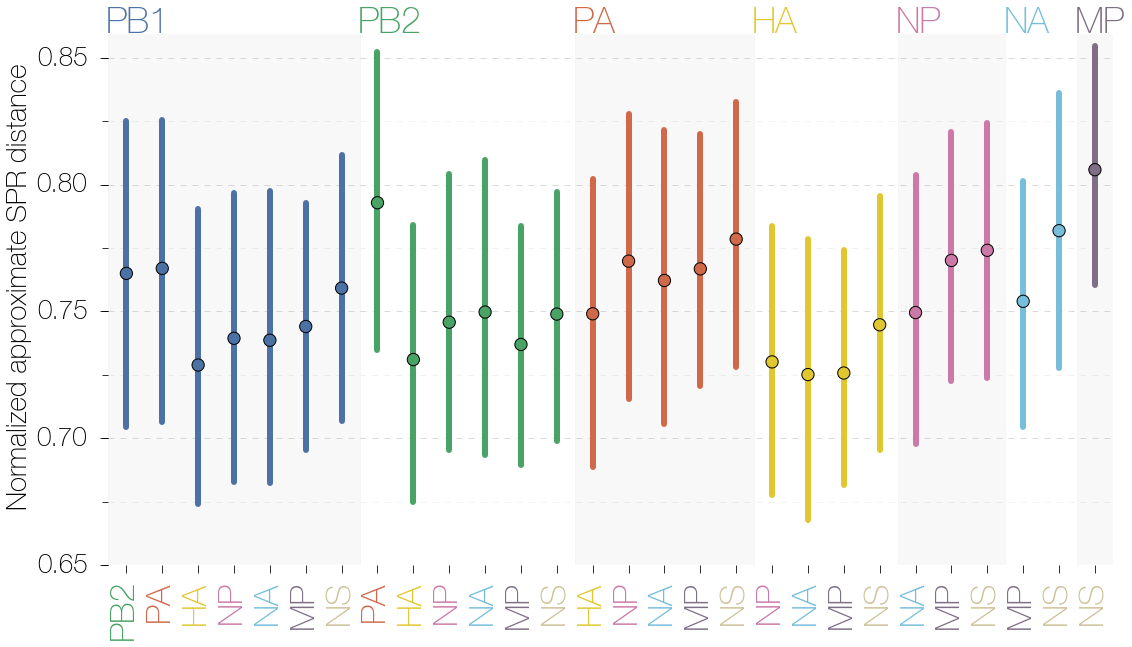
\includegraphics[width=0.65\textwidth]{supp_figures/InfB_normalizedApproxSPR.png}
	\caption{\textbf{Normalized approximate SPR distances between pairs of segments.}
Following the normalization procedure approximate SPR distances are similar across all pairwise comparisons.
We interpret this as lack of evidence for small-scale topological similarities between trees of all segments, which we expect to arise if any two segments were being co-packaged and co-reassorted.
All vertical lines indicating uncertainty are 95\% highest posterior densities (HPDs).}
	\label{SPRdistances}
\end{figure}

The 95\% highest posterior density (HPD) intervals of normalized approximate SPR distances between pairs of segments encompass most means and occupy a relatively small range, suggesting there is no evidence of differences in the number of reassortments between segments (Figure \ref{SPRdistances}).
Reassortment rate given as number of SPR moves per total time in both trees shows similar results (Figure \ref{NormSPR_RErate}).
This is in line with recent experiments in influenza A that have shown that reassortment between segments differing by a single synonymous difference is highly efficient \citep{marshall2013}.
We note, however, that because of phylogenetic uncertainty our estimate of SPR distance might simply lack power.
Comparisons between independent analyses of the same segments yield distances that are comparable to distances between different segments (Figures \ref{SPRdistancesTrees} and \ref{SPRdistancesReplicates}), suggesting that phylogenetic uncertainty is making a considerable contribution to our estimates of approximate SPR distances.
Still, we find that independent replicates from the same segment (Figure \ref{SPRdistancesReplicates}) show lower SPR distances that comparisons between segments (Figure \ref{SPRdistancesTrees}), suggesting that phylogenetic noise is not completely overwhelming reassortment signal.
In addition, SPR distances themselves can only approximate (and underestimate) the actual numbers of reassortments.
Thus we caution against over-interpreting Figure \ref{SPRdistances}.
Although there might be concern about using approximate, rather than exact, SPR distances we do estimate exact SPR distances for a limited number of segment pairs - PB1, PB2 and HA - and find that after normalization exact and approximate SPR distances are not significantly different (Figures \ref{NormSPR_PB1-PB2_difference}--\ref{NormSPR_PB2-HA_difference}).


\begin{figure}
\centering  
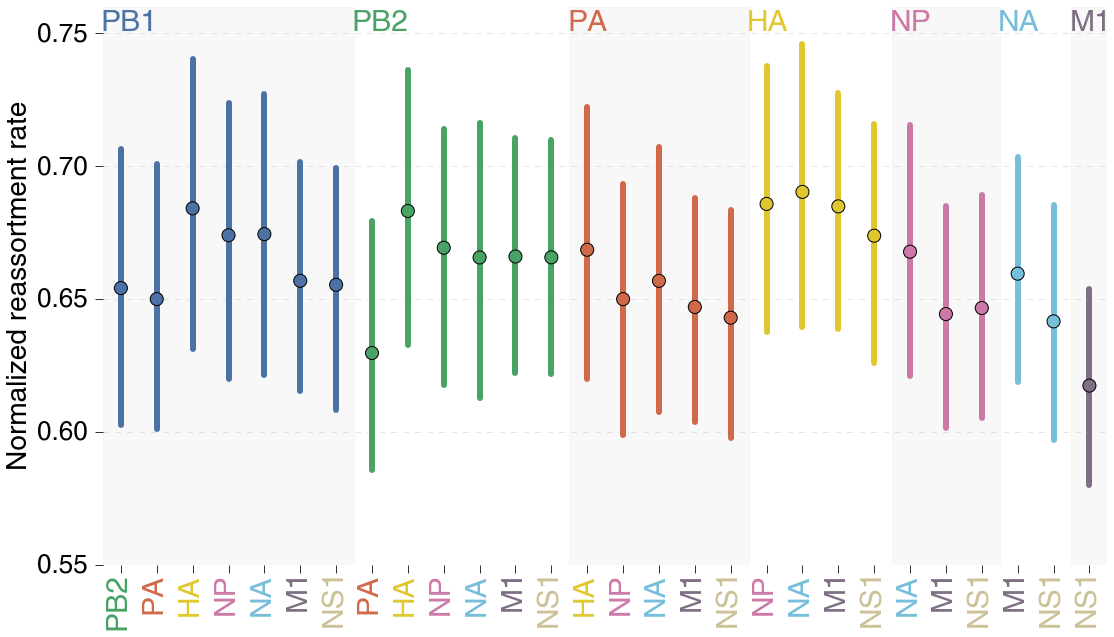
\includegraphics[width=0.65\textwidth]  {supp_figures/InfB_supp_normRErate.png}
\caption{\textbf{Normalized reassortment rate}
Reassortment rate is calculated as approximate number of SPR moves per sum of total time in both trees.}
\label{NormSPR_RErate}
\end{figure}

\begin{figure}
\centering  
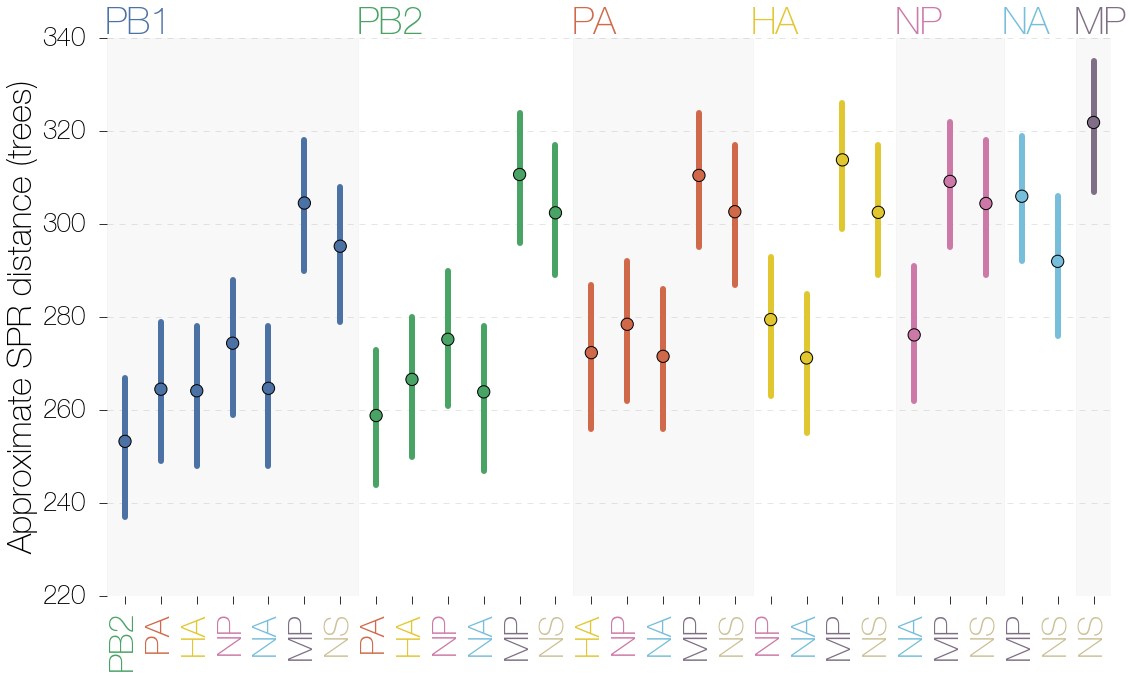
\includegraphics[width=0.65\textwidth]  {supp_figures/InfB_supp_aSPRdistances_trees.png}
\caption{\textbf{Approximate SPR distances between all pairs of trees of segments.}
There is a visible trend where comparisons between shorter segments have larger SPR distances, consistent with decreasing tree topology stability over the course of MCMC for shorter segments.}
\label{SPRdistancesTrees}
\end{figure}

\begin{figure}
\centering  
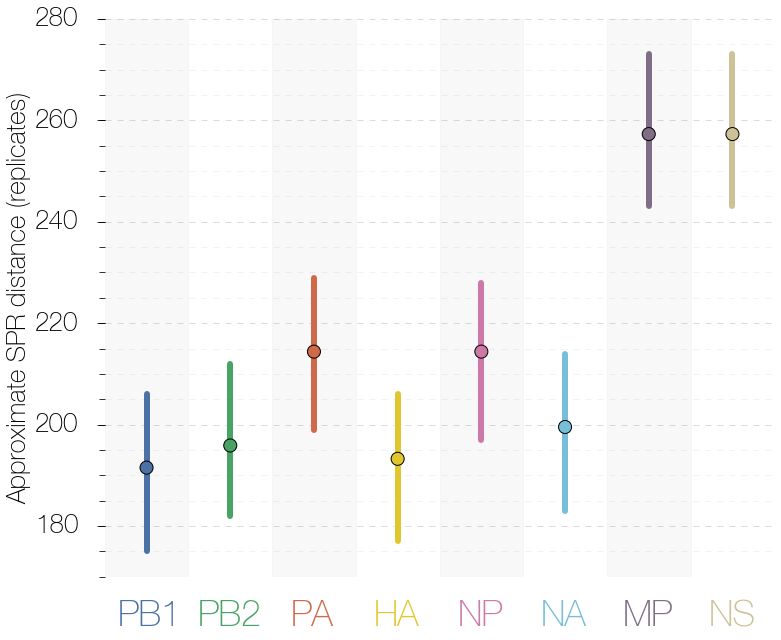
\includegraphics[width=0.65\textwidth]  {supp_figures/InfB_supp_aSPRdistances_replicates.png}
\caption{\textbf{Approximate SPR distances between replicate trees of each segment.}
Approximate SPR distances between replicates of MP and NS trees are much higher ($\approx$260) than any other segments, suggesting greater variability in tree topology over the course of MCMC.
SPR distances between replicates of most other segments are $\approx$200.
}
\label{SPRdistancesReplicates}
\end{figure}

\begin{figure}
\centering  
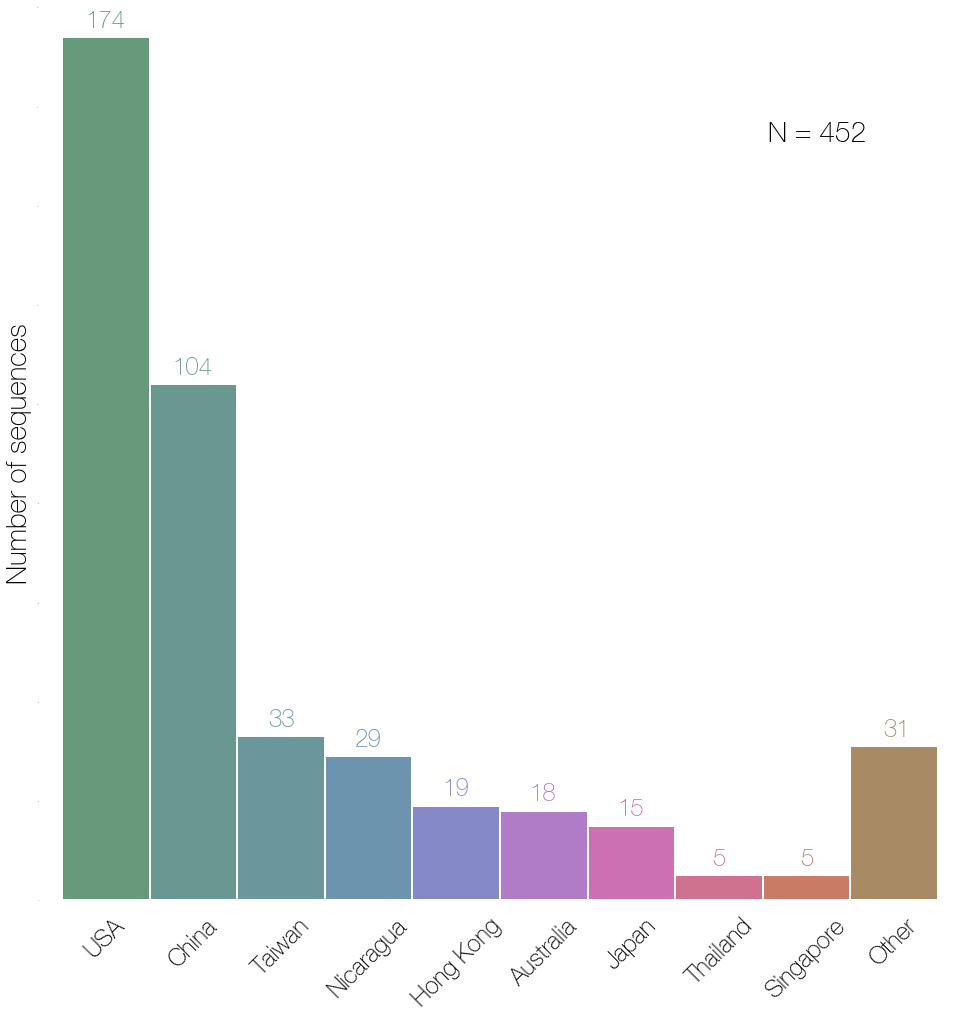
\includegraphics[width=0.45\textwidth]  {supp_figures/InfB_seqCountries.452.png}
\caption{\textbf{Geographic distribution of sequences in the primary dataset.}
Sequences were assigned to the ``other'' category if there were less than 5 sequences from that country.
Most of the genomes in the primary dataset were sampled in the USA.}
\label{geoSeqs4}
\end{figure}

\begin{figure}
\centering  
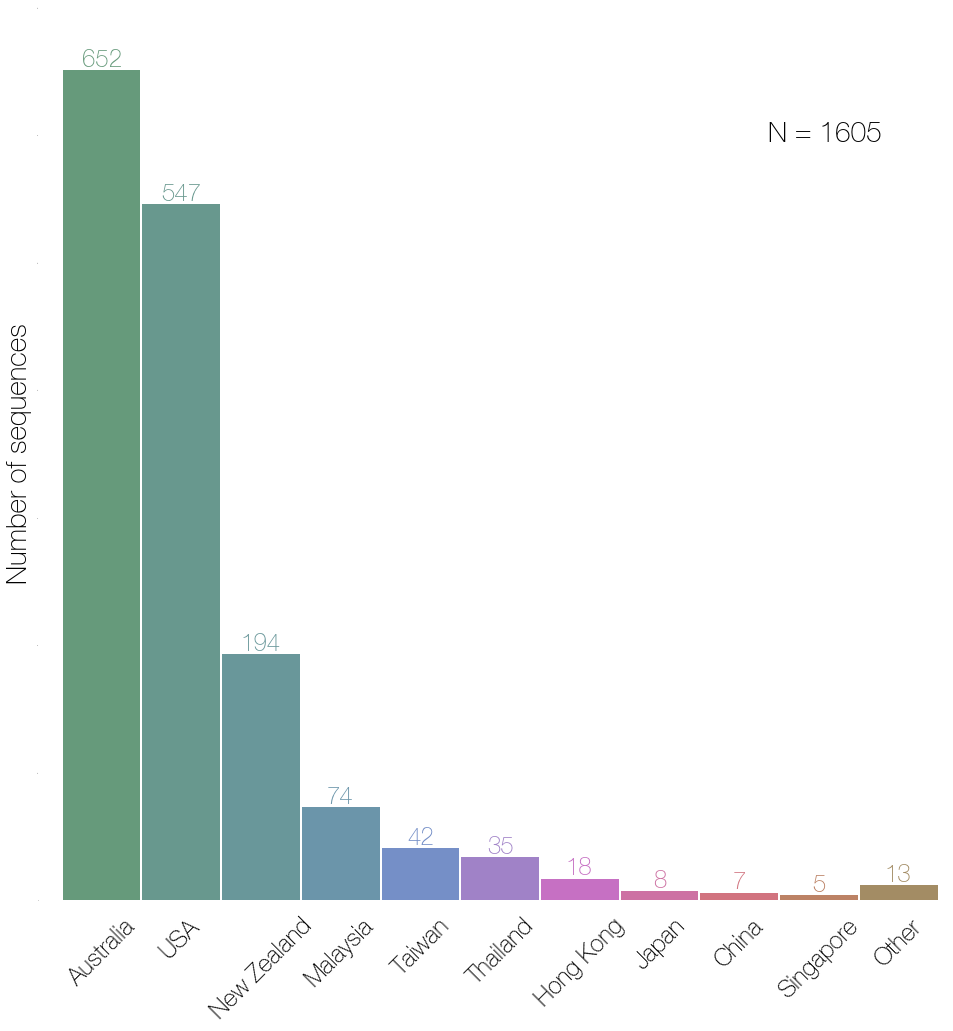
\includegraphics[width=0.45\textwidth]  {supp_figures/InfB_seqCountries.1600.png}
\caption{\textbf{Geographic distribution of sequences in the secondary dataset.}
Sequences were assigned to the ``other'' category if there were less than 5 sequences from that country.
Most of the genomes in the secondary dataset were sampled in Australia.}
\label{geoSeqs1600}
\end{figure}

\begin{figure}
\centering  
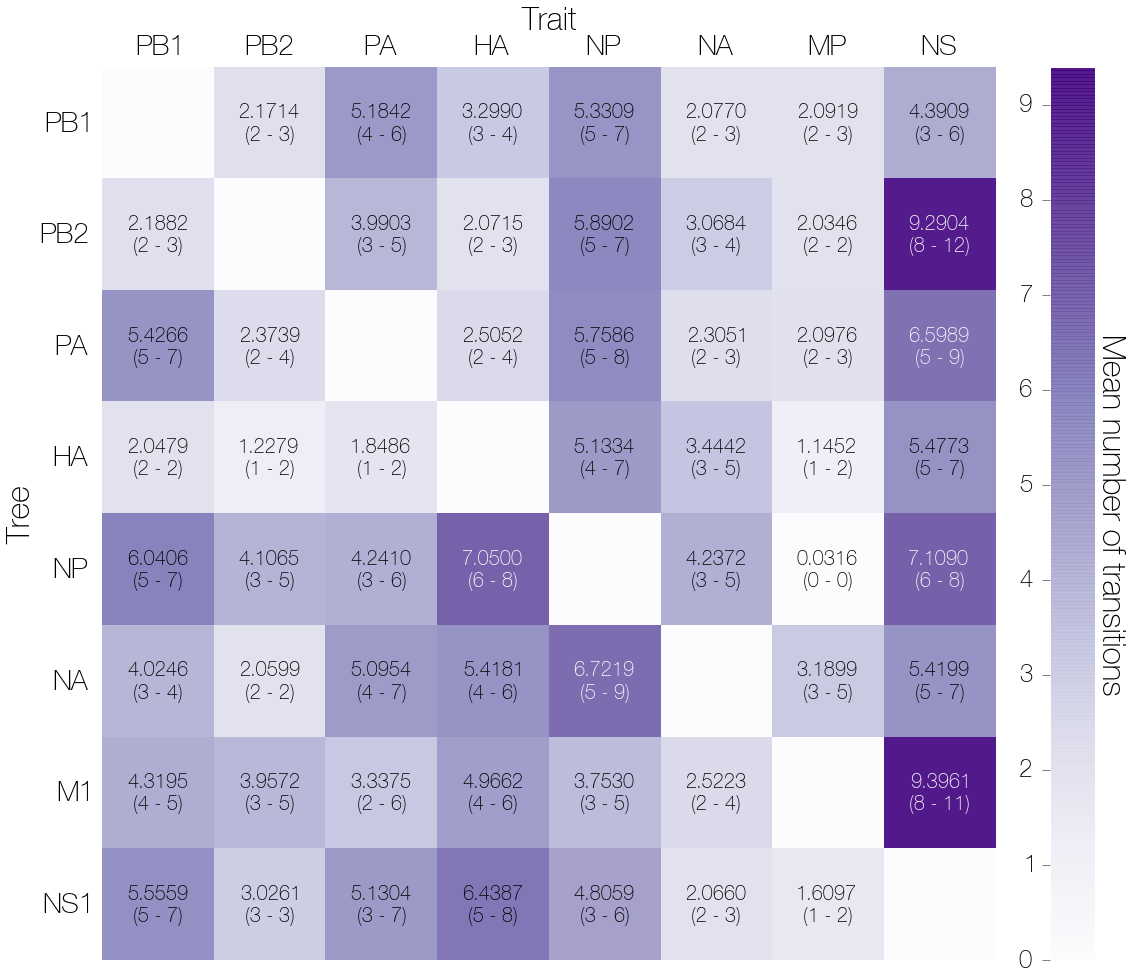
\includegraphics[width=0.75\textwidth]  {supp_figures/InfB_Ntransitions.png}
\caption{\textbf{Numbers of trait transitions in each tree.}
The numbers shown are the mean inferred number of trait transitions (minus one to account for the initial Vic--Yam split) in a given tree and trait combination.
The numbers in brackets correspond to 95\% highest posterior density intervals.
Transitions may not be independent when more than one segment reassorts at the same time.}
\label{Ntransitions}
\end{figure}

\begin{figure}
\centering  
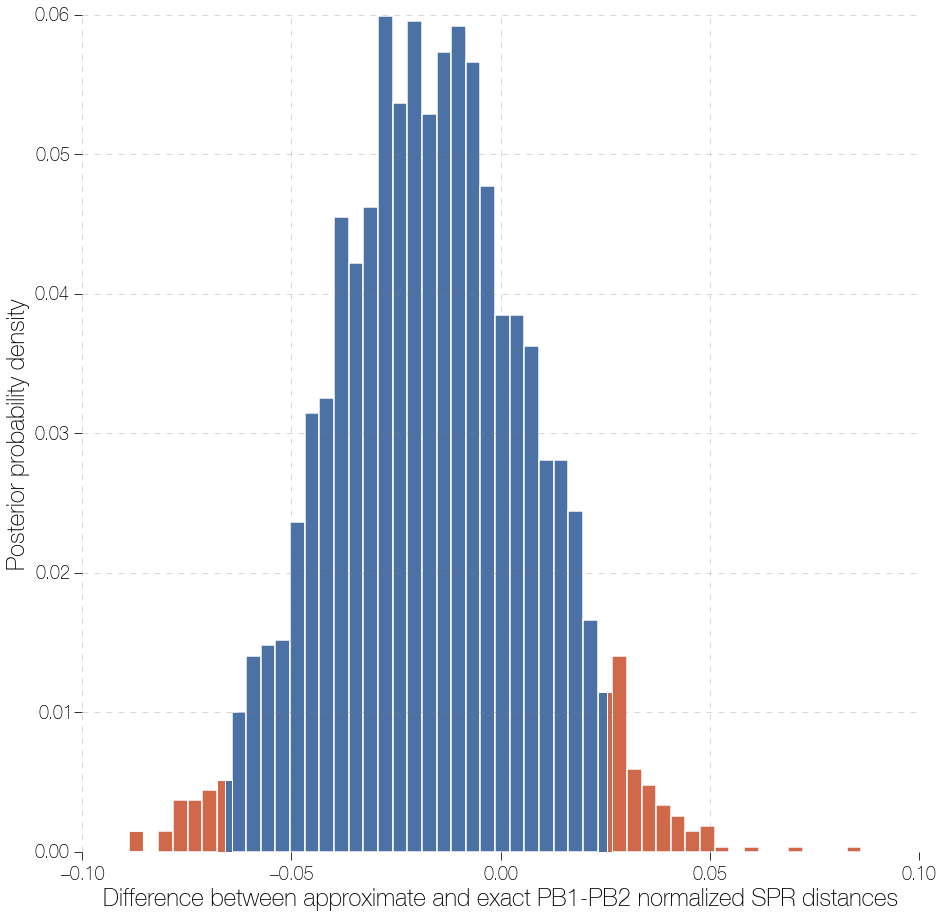
\includegraphics[width=0.65\textwidth]  {supp_figures/InfB_supp_NormPB1-PB2_hist.png}
\caption{\textbf{Distribution of differences between exact and approximate PB1-PB2 SPR distances after normalization.}
95\% HPD interval (blue) overlaps zero, suggesting no evidence of differences between approximate and exact SPR distances following normalization.}
\label{NormSPR_PB1-PB2_difference}
\end{figure}

%\begin{figure}
%\centering  
%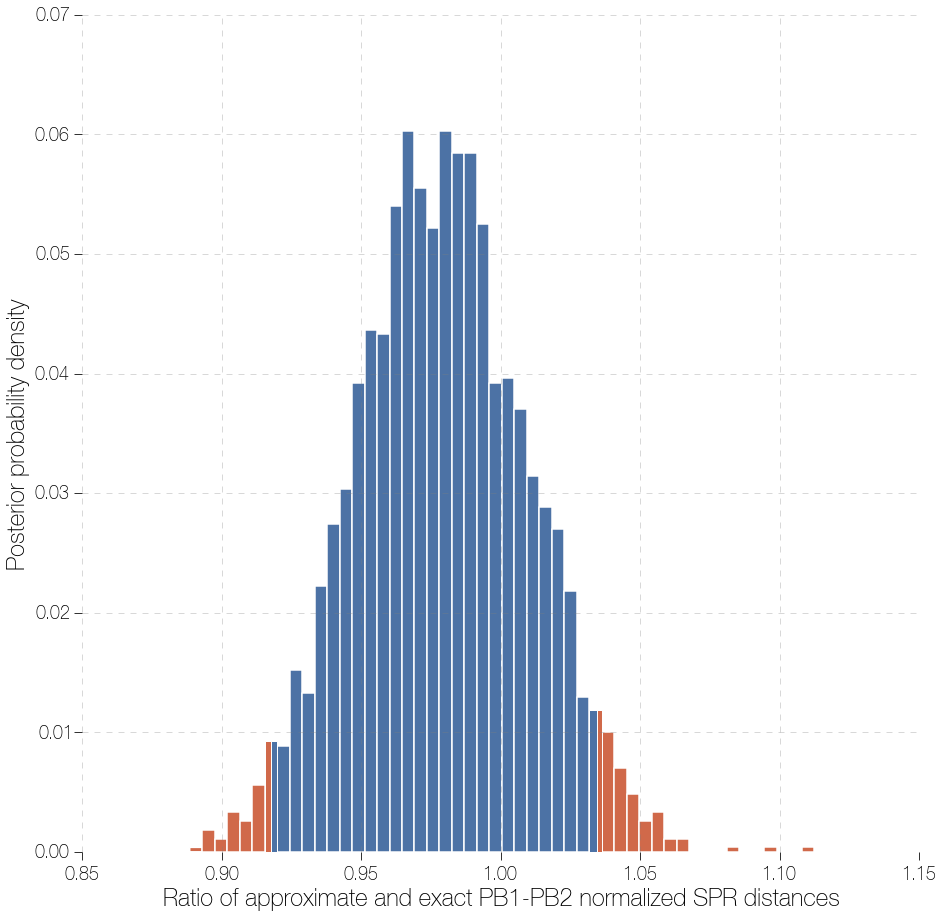
\includegraphics[width=0.65\textwidth]  {supp_figures/InfB_supp_NormPB1-PB2_hist2.png}
%\caption{\textbf{Distribution of ratios between exact and approximate PB1-PB2 SPR distances after normalization.}
%95\% HPD interval (blue) overlaps 1, suggesting no evidence of differences between approximate and exact SPR distances following normalization.}
%\label{NormSPR_PB1-PB2_ratio}
%\end{figure}

\begin{figure}
\centering  
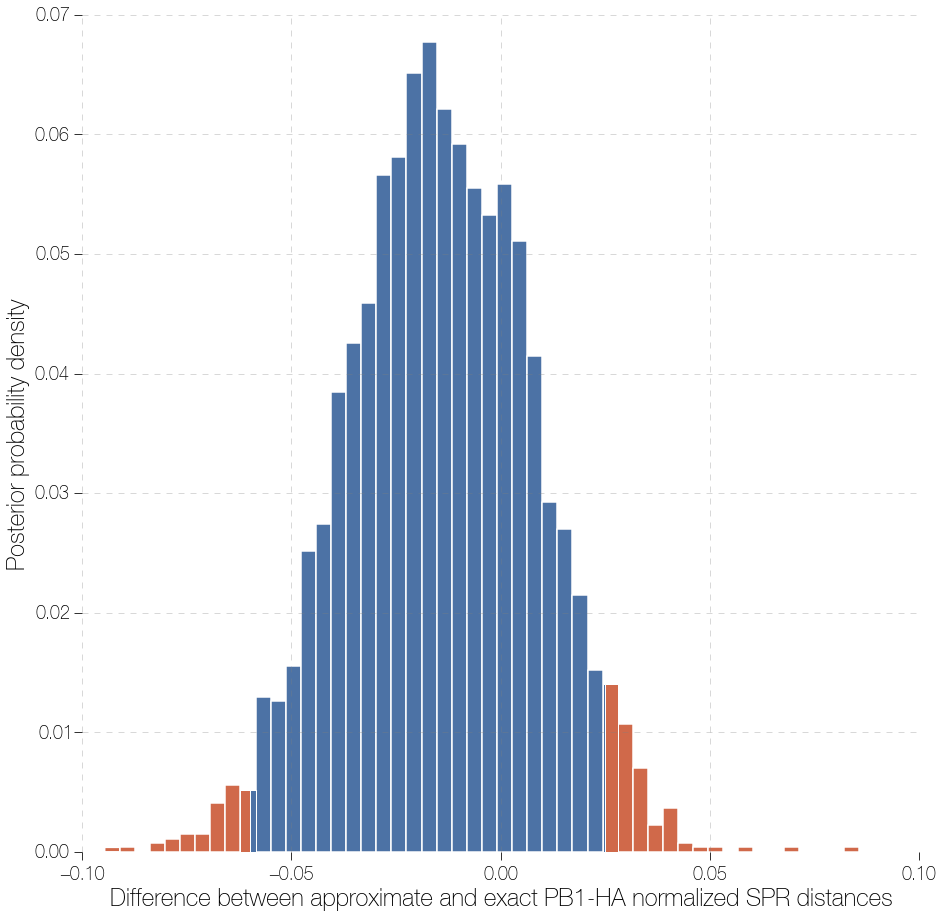
\includegraphics[width=0.65\textwidth]  {supp_figures/InfB_supp_NormPB1-HA_hist.png}
\caption{\textbf{Distribution of differences between exact and approximate PB1-HA SPR distances after normalization.}
95\% HPD interval (blue) overlaps zero, suggesting no evidence of differences between approximate and exact SPR distances following normalization.}
\label{NormSPR_PB1-HA_difference}
\end{figure}

%\begin{figure}
%\centering  
%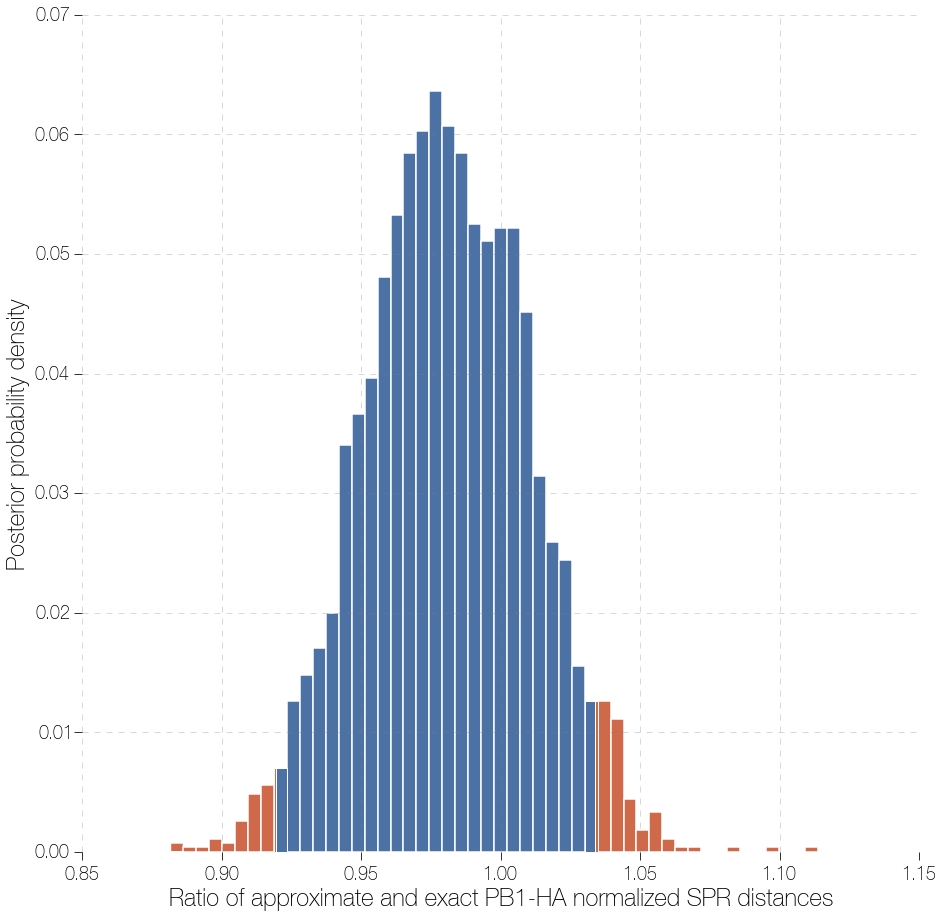
\includegraphics[width=0.65\textwidth]  {supp_figures/InfB_supp_NormPB1-HA_hist2.png}
%\caption{\textbf{Distribution of ratios between exact and approximate PB1-HA SPR distances after normalization.}
%95\% HPD interval (blue) overlaps 1, suggesting no evidence of differences between approximate and exact SPR distances following normalization.}
%\label{NormSPR_PB1-HA_ratio}
%\end{figure}

\begin{figure}
\centering  
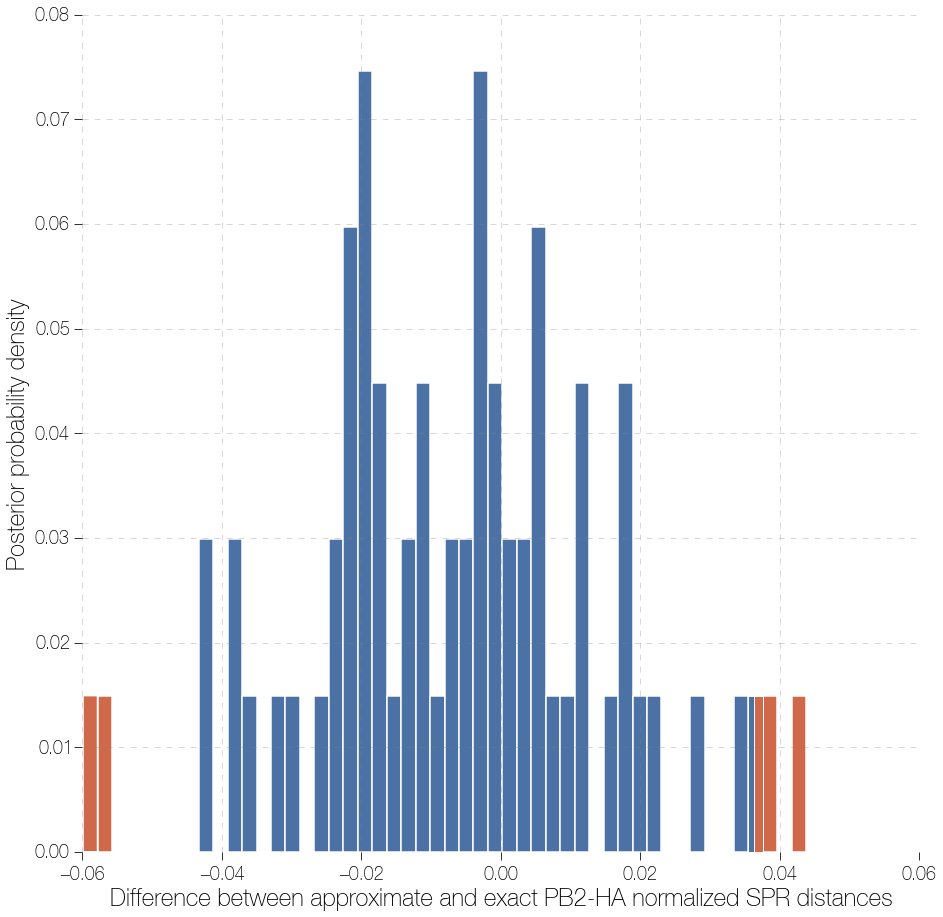
\includegraphics[width=0.65\textwidth]  {supp_figures/InfB_supp_NormPB2-HA_hist.png}
\caption{\textbf{Distribution of differences between exact and approximate PB2-HA SPR distances after normalization.}
95\% HPD interval (blue) overlaps zero, suggesting no evidence of differences between approximate and exact SPR distances following normalization.
Due to excessively long computation time of exact SPR distances between PB2 and HA trees few comparisons were made.}
\label{NormSPR_PB2-HA_difference}
\end{figure}

%\begin{figure}
%\centering  
%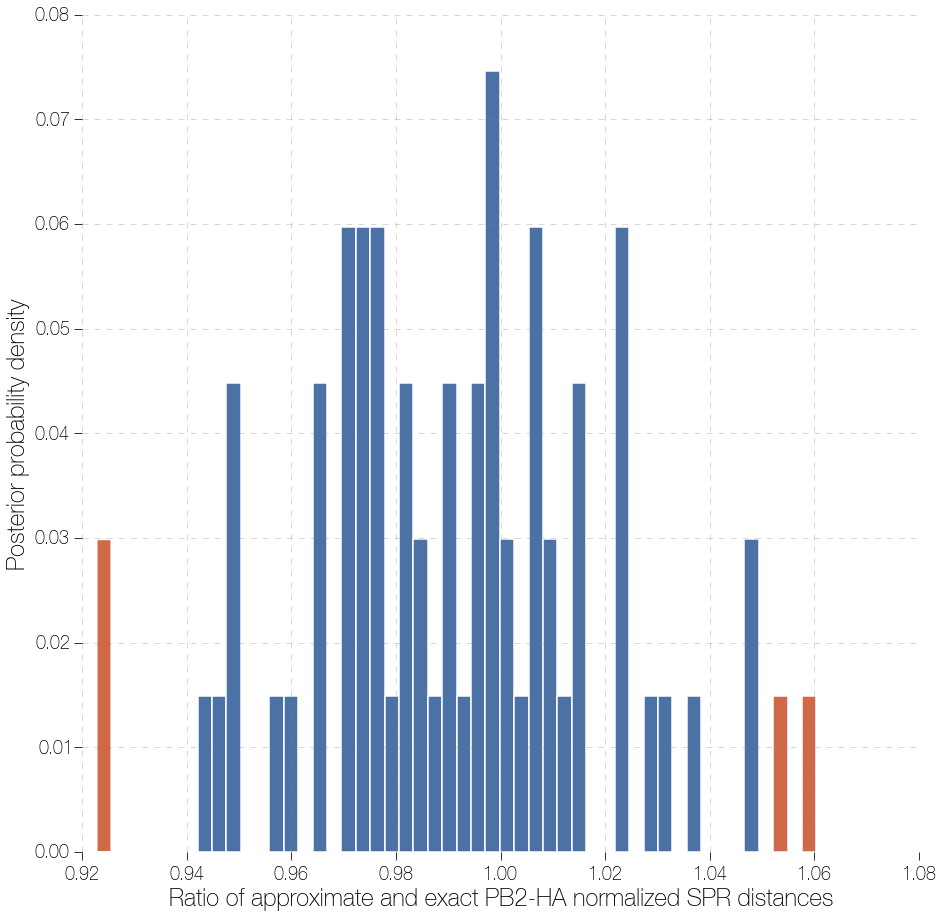
\includegraphics[width=0.65\textwidth]  {supp_figures/InfB_supp_NormPB2-HA_hist2.png}
%\caption{\textbf{Distribution of ratios between exact and approximate PB2-HA SPR distances after normalization.}
%95\% HPD interval (blue) overlaps 1, suggesting no evidence of differences between approximate and exact SPR distances following normalization.
%Due to excessively long computation time of exact SPR distances between PB2 and HA trees few comparisons were made.}
%\label{NormSPR_PB2-HA_ratio}
%\end{figure}

\begin{figure}
\centering  
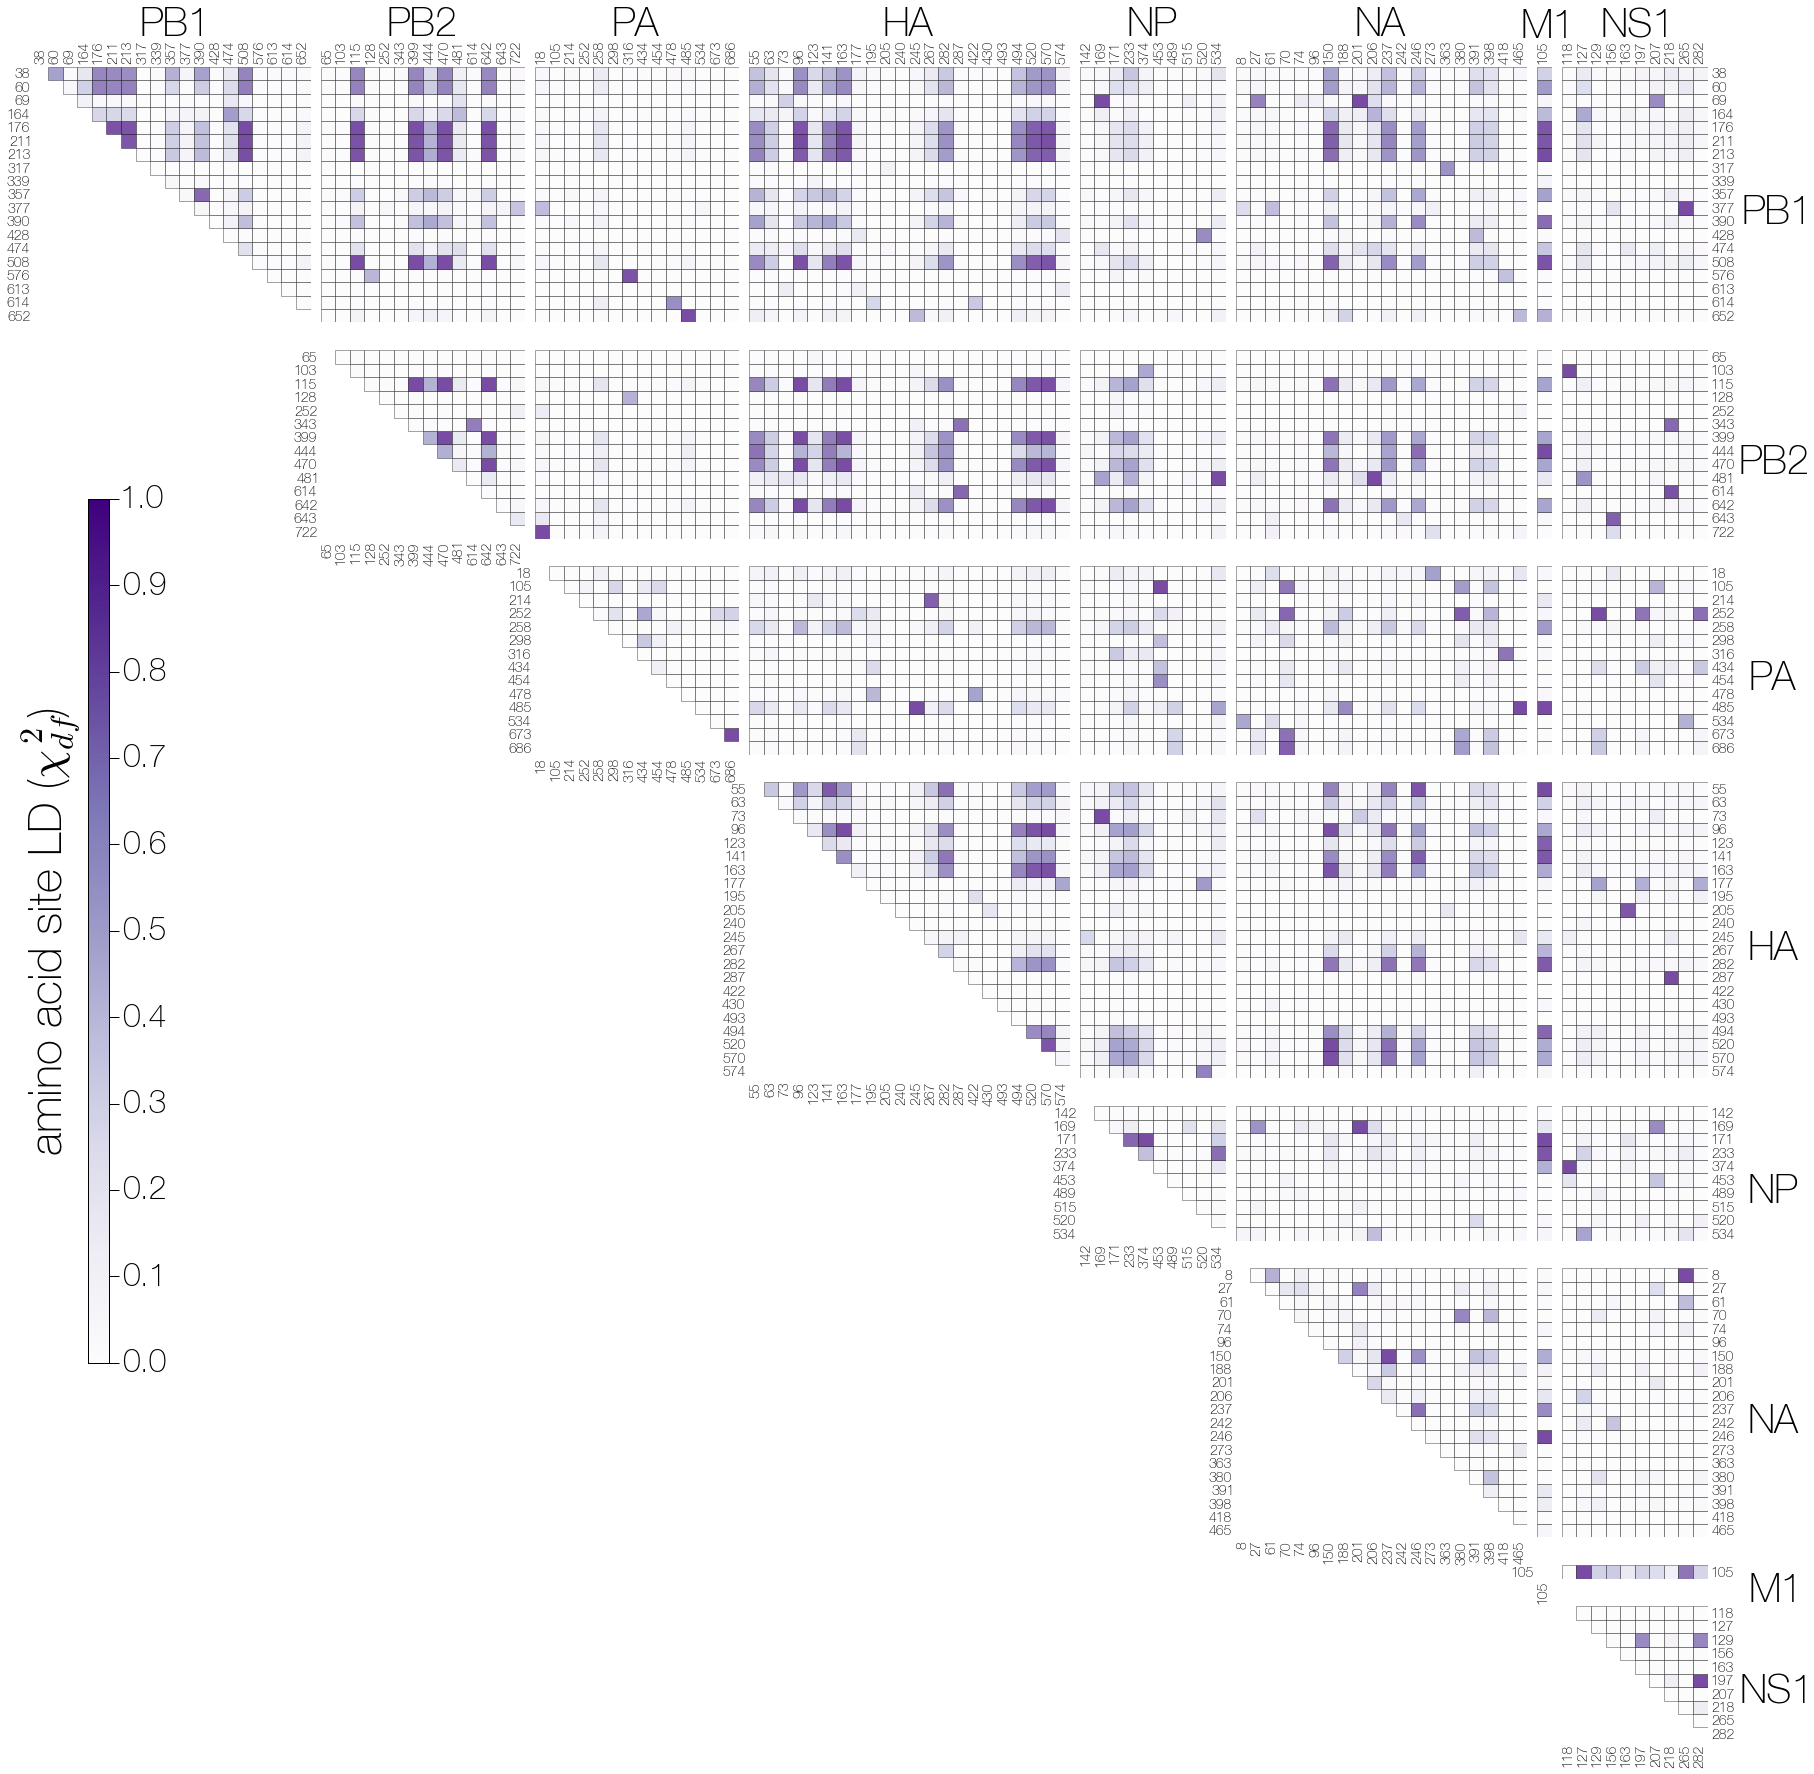
\includegraphics[width=0.95\textwidth]  {supp_figures/InfB_LDheatmap.1600.aa.ChiSqdf.minorCutoff1percent.png}
\caption{\textbf{Heatmap of genome-wide linkage disequilibrium ($\chiSq$) between polymorphic amino acid sites.}
Patterns of LD across the genome suggest a network of reciprocally linked amino acid sites on PB1, PB2, HA and, to some extent NA, proteins.
Proximity of sites on heatmaps might not correspond to proximity of sites within proteins.}
\label{ChiGenome}
\end{figure}

\begin{figure}
\centering  
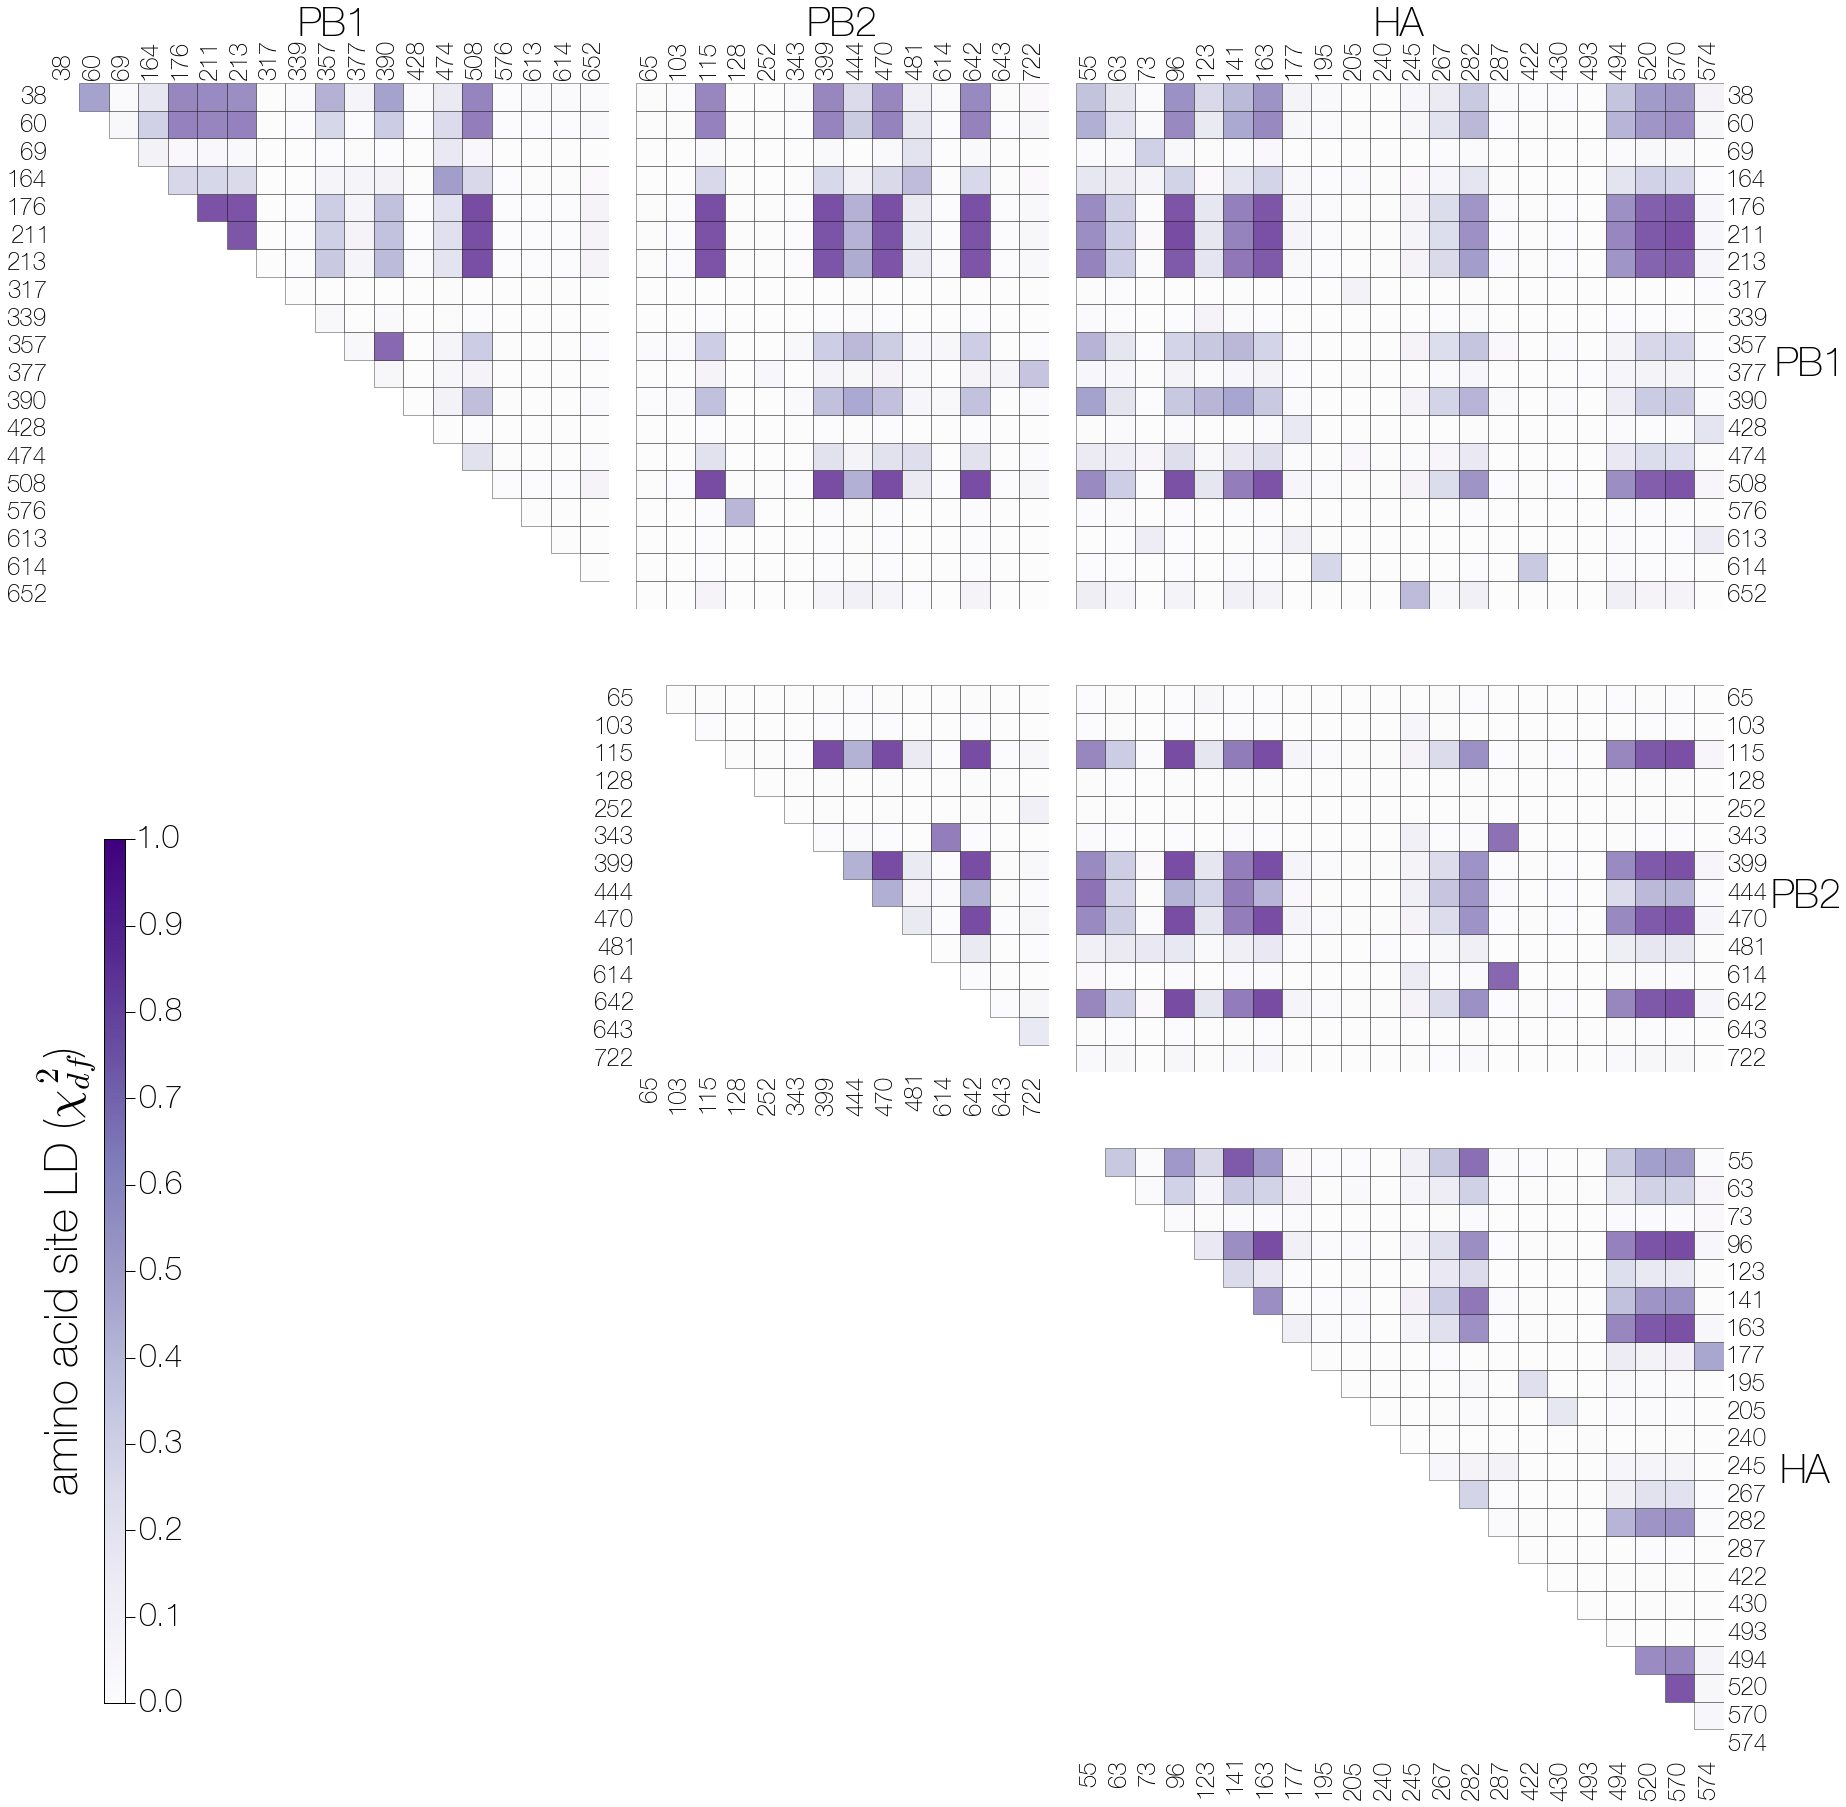
\includegraphics[width=0.85\textwidth]  {supp_figures/InfB_LDheatmap.PB1_PB2_HA.1600.aa.ChiSqdf.minorCutoff1percent.png}
\caption{\textbf{Heatmap of linkage disequilibrium ($\chiSq$) between amino acid sites on PB1, PB2 and HA proteins.}
Numbers next to each row and column correspond to amino acid site number within a given protein starting from methionine.
Amino acid sites exhibiting reciprocally high LD between PB1, PB2 and HA proteins are: 176, 211, 213, 508 (PB1), 115, 399, 470, 642 (PB2) and 96, 163, 520 and 570 (HA).
Sites 211 and 213 on the PB1 protein are very close to each other and the stretch of sequence around these residues contains many positively charged amino acids (lysine and arginine).
Multiple nuclear localization signals (NLSs) are predicted to occur around this region and sites 211 and 213 are either predicted to be near the end of a mono-partite NLS or the beginning of a bi-partite NLS.
Previous research \citep{nath1990} suggests that in the influenza A PB1 protein residue 211 (homologous to influenza B PB1 residue 211) is the last residue of a bi-partite NLS.
Almost all Yamagata lineage isolates possess arginine (R) residue at PB1 position 211 and a serine (S) residue at position 213, whereas Victoria lineage isolates have lysine (K) at position 211 and threonine (T) at position 213.
It remains to be seen whether these sites significantly affect the nuclear import efficiency of the PB1 protein of either lineage.
Though the PB1 protein is known to accumulate in the nucleus on its own, efficient import into the nucleus requires the presence of the PA protein \citep{fodor2004}.
Similarly, site 399 on the PB2 protein are close to residues 377, 406 and 408 which are homologous to sites in influenza A that are responsible for mRNA cap-binding \citep{guilligay2008}.}
\label{ChiCore}
\end{figure}

\begin{figure}
\centering  
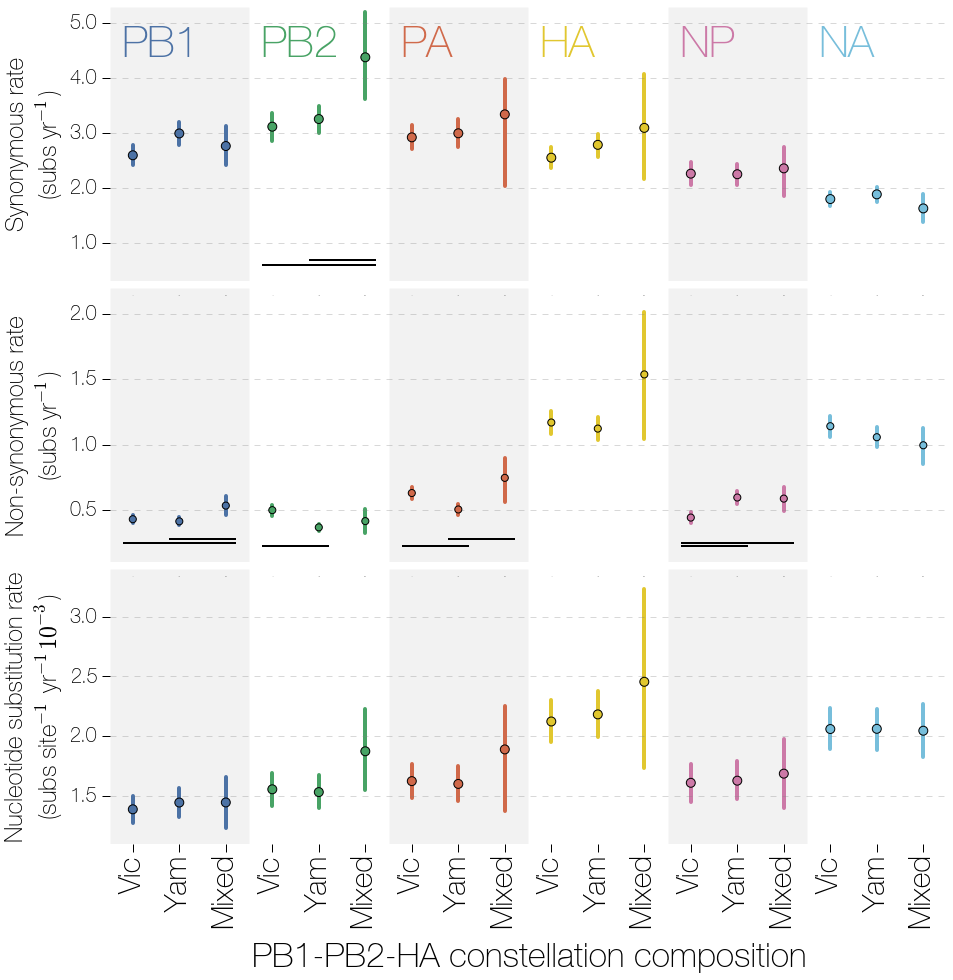
\includegraphics[width=0.65\textwidth]  {supp_figures/InfB_robustCounting.png}
\caption{\textbf{Synonymous, non-synonymous and nucleotide substitution rates in segments under different PB1-PB2-HA complexes.}
Evolutionary rate dissimilarities under Vic and Yam PB1-PB2-HA complexes are not systematic and appear negligible.
Synonymous and non-synonymous rates were calculated by dividing the sum of all substitutions of a given class by the total amount of evolutionary time under each PB1-PB2-HA constellation.
Nucleotide rates were calculated by multiplying the inferred nucleotide substitution rate on each branch by the branch length, then dividing this by the total amount of evolutionary time under each PB1-PB2-HA constellation.
Vertical bars indicating uncertainty are 95\% HPDs, black bars indicate 95\% HPDs that do not overlap.}
\label{robustCounting}
\end{figure}

%Figures \ref{SPRdistancesTrees} and \ref{SPRdistancesReplicates} are showing approximate SPR distances prior to the normalization procedure (see Methods).
%Figure \ref{SPRdistancesTrees} shows that MP and NS trees show greater approximate SPR distances when compared to any other segment tree, which is consistent with the fact that only M1 and NS1 coding sequences, which are shorter than any %other coding sequences, were used to infer the trees.
%Figure \ref{SPRdistancesReplicates} confirms this by showing greater variability in tree topology (as greater approximate SPR distance) when MP and NS trees are compared against their replicates.
%For all other segments approximate SPR distances between all pairs of trees prior to normalization suggests that most segment pairs have similar posterior distributions of approximate SPR distances.

%Figures \ref{deltaTMRCAtrees} and \ref{deltaTMRCAreplicates} show $\dtmrca$ statistics for inter-segment and intra-segment, respectively, comparisons prior to normalization.
%Figure \ref{deltaTMRCAtrees} shows that similarity in TMRCAs (as low $\dtmrca$) between PB1, PB2 and HA segments is due to considerably smaller $\dtmrca$ statistic for the comparison between these segments.
%It is also noteworthy that NA and MP comparisons have similarly low values for this statistic.
%Figure \ref{deltaTMRCAreplicates} shows that TMRCAs are quite robust over the course of MCMC and node times do not, even in the most extreme cases, deviate from their replicates by more than 1 year.

\begin{figure}
\centering  
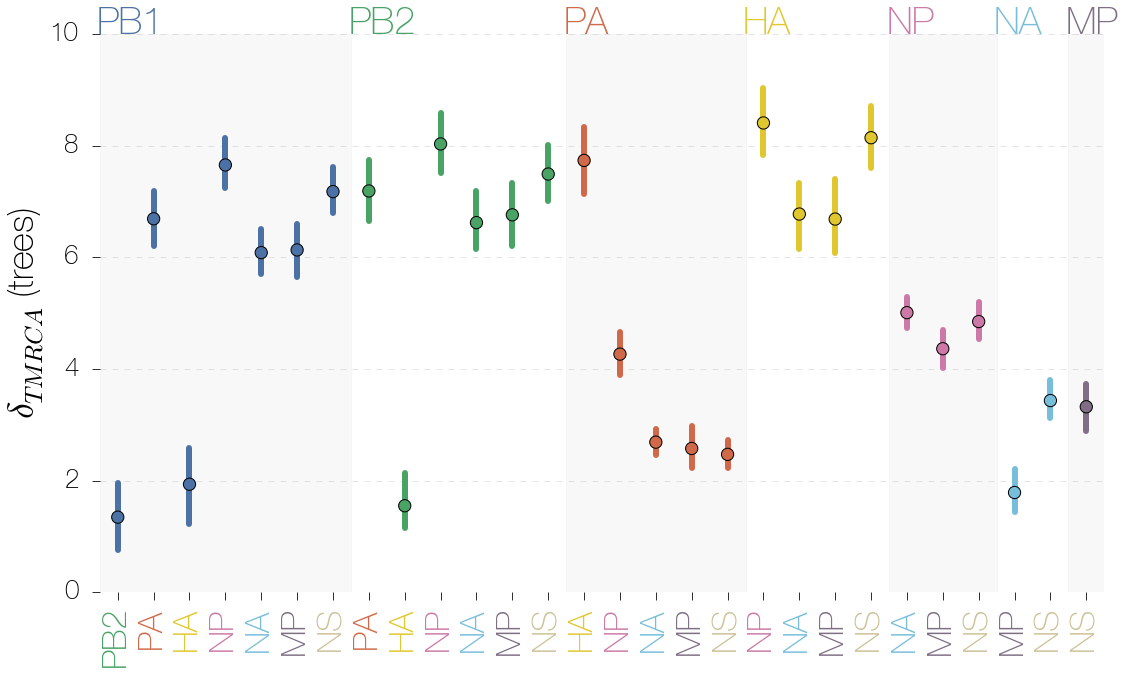
\includegraphics[width=0.65\textwidth]  {supp_figures/InfB_supp_deltaTMRCA_trees.png}
\caption{\textbf{Mean $\dtmrca$ between all pairs of trees of segments.}
Mean $\dtmrca$ between trees of segments reveal that tip pairs in PB1, PB2 and HA trees have very similar TMRCAs.
The upper tail of the 95\% HPD (HPDs are represented as vertical lines) interval of mean $\dtmrca$ values for PB1-PB2-HA and MP-NA trees do not exceed 3 years.}
\label{deltaTMRCAtrees}
\end{figure}

\begin{figure}
\centering  
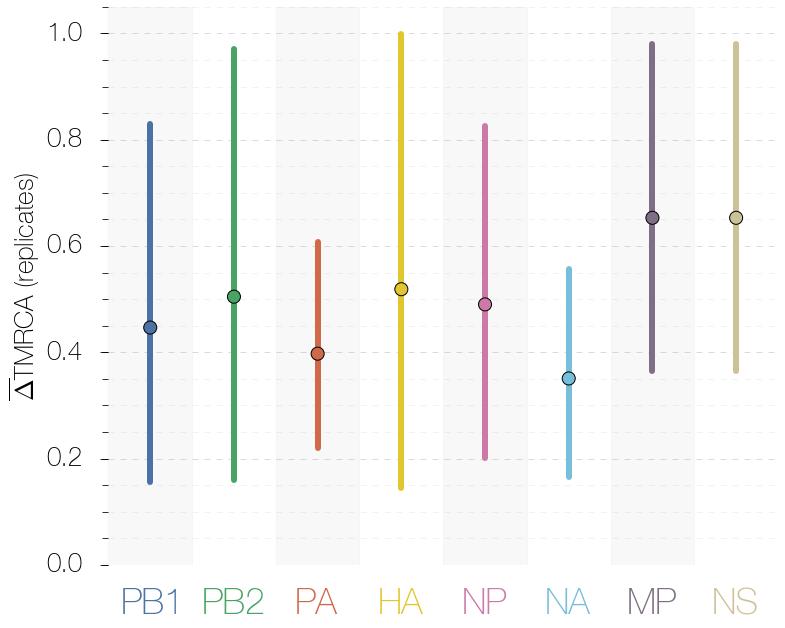
\includegraphics[width=0.65\textwidth]  {supp_figures/InfB_supp_deltaTMRCA_replicates.png}
\caption{\textbf{Mean $\dtmrca$ between replicate trees of each segment.}
Mean $\dtmrca$ values between independent analyses of each segment show that mean $\dtmrca$ values rarely exceed 1 year.}
\label{deltaTMRCAreplicates}
\end{figure}

%We also tested the accuracy of approximate SPR distances using exact SPR distances calculated from PB1, PB2 and HA comparisons.
%Figures \ref{SPR_PB1-PB2_difference}--\ref{SPR_PB2-HA_ratio} show that after normalization the approximate and exact SPR distance estimates are not significantly different.
%There is also good correlation between the two SPR distances (Figures \ref{SPR_PB1-PB2_correlation}--\ref{SPR_PB2-HA_correlation}). 
%Due to excessively long computation time of exact SPR distances very few PB2--HA comparisons were made.

%\begin{figure}
%\centering  
%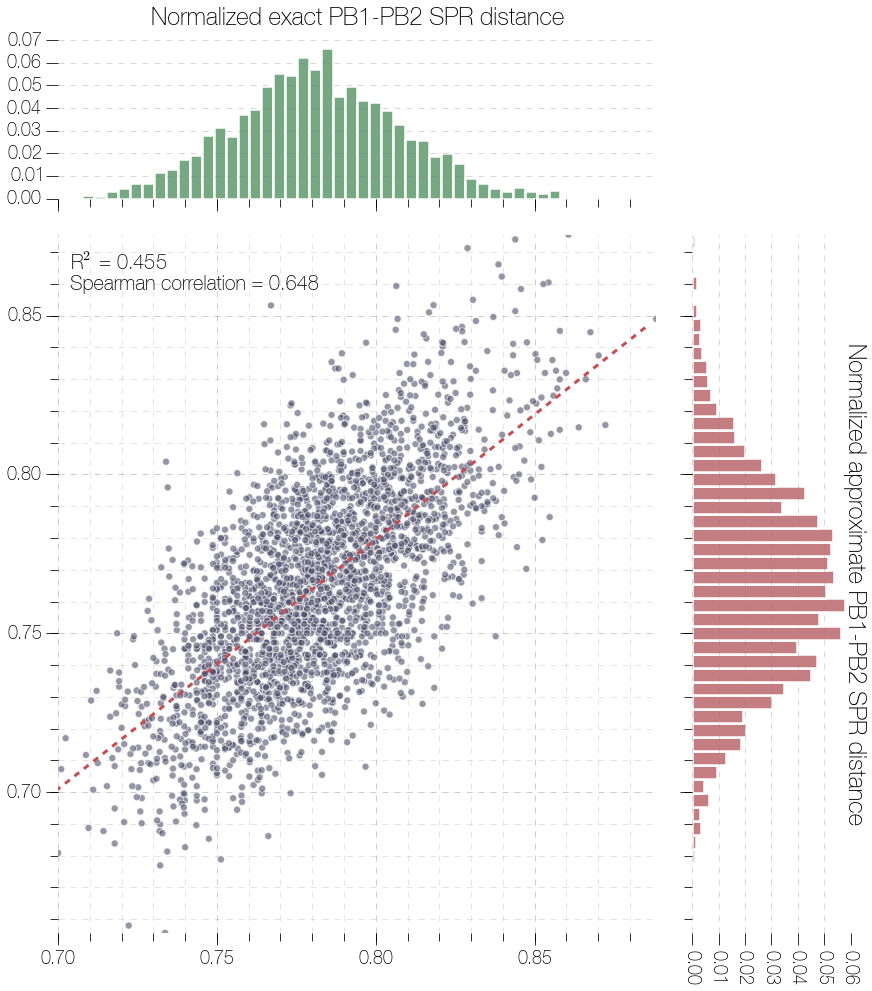
\includegraphics[width=0.5\textwidth]  {supp_figures/InfB_supp_NormPB1-PB2_corr.png}
%\caption{\textbf{Correlation between exact and approximate PB1-PB2 SPR distances after normalization.}}
%\label{NormSPR_PB1-PB2_correlation}
%\end{figure}

%\begin{figure}
%\centering  
%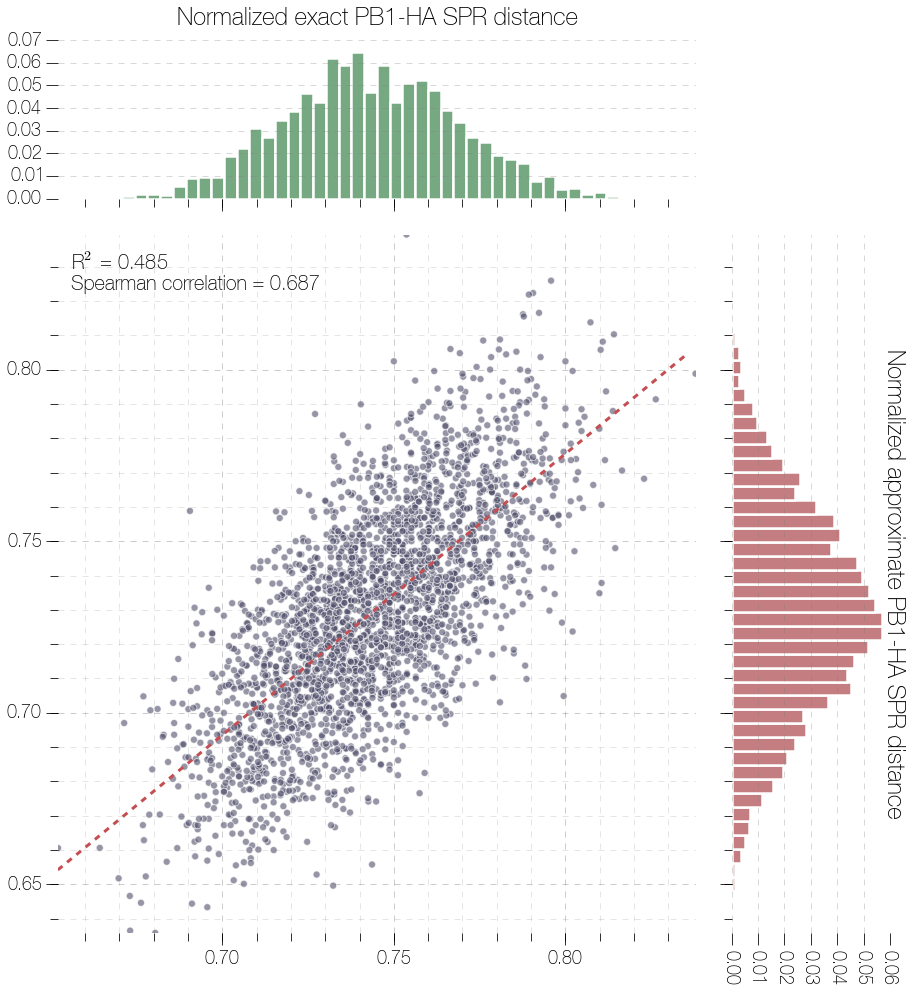
\includegraphics[width=0.5\textwidth]  {supp_figures/InfB_supp_NormPB1-HA_corr.png}
%\caption{\textbf{Correlation between exact and approximate PB1-HA SPR distances after normalization.}}
%\label{NormSPR_PB1-HA_correlation}
%\end{figure}

%\begin{figure}
%\centering  
%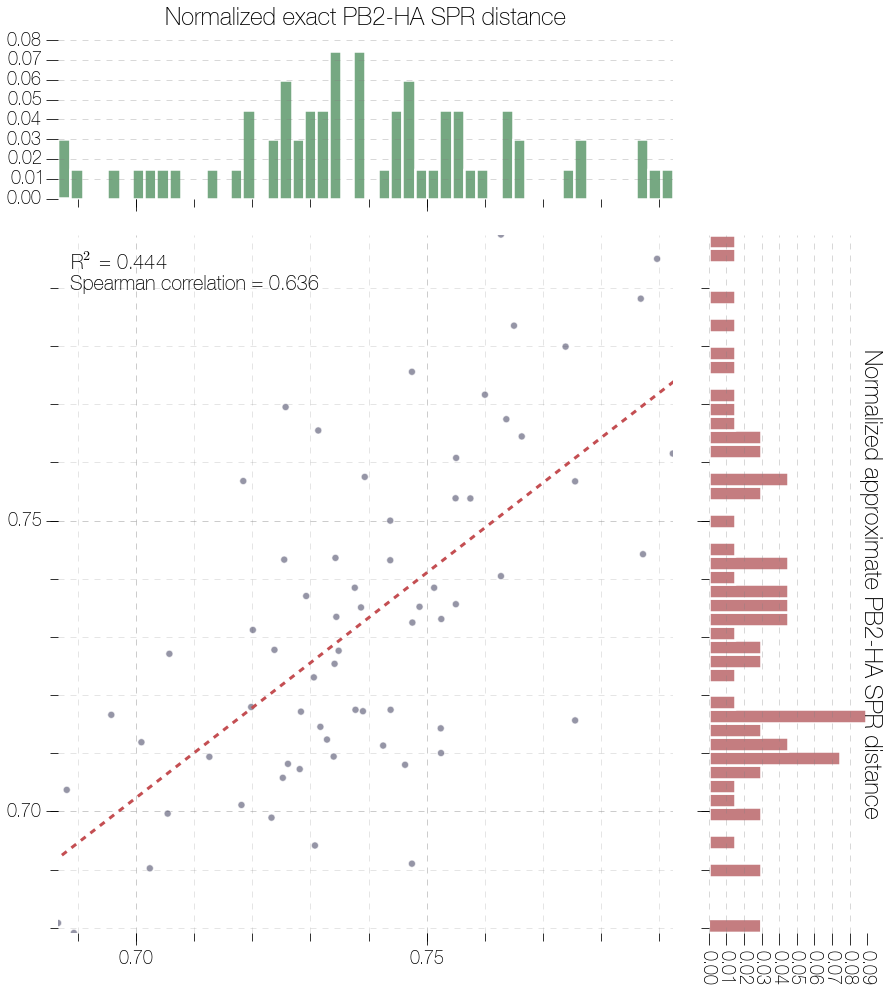
\includegraphics[width=0.5\textwidth]  {supp_figures/InfB_supp_NormPB2-HA_corr.png}
%\caption{\textbf{Correlation between exact and approximate PB2-HA SPR distances after normalization.}
%Due to excessively long computation time of exact SPR distances between PB2 and HA trees few comparisons were made.}
%\label{NormSPR_PB2-HA_correlation}
%\end{figure}

%Figures \ref{SPR_PB1-PB2_difference}--\ref{SPR_PB2-HA_ratio} focus on differences between exact and approximate SPR distances and show that prior to normalization approximate SPR distances are overestimates of exact SPR distances.
%Figures \ref{SPR_PB1-PB2_correlation}--\ref{SPR_PB2-HA_correlation} show that there is a similar degree of correspondence between approximate and exact SPR distances to when approximate and exact SPR distances are normalized (Figures %\ref{NormSPR_PB1-PB2_correlation}--\ref{NormSPR_PB2-HA_correlation}) using the procedure described in Methods.

%\begin{figure}
%\centering  
%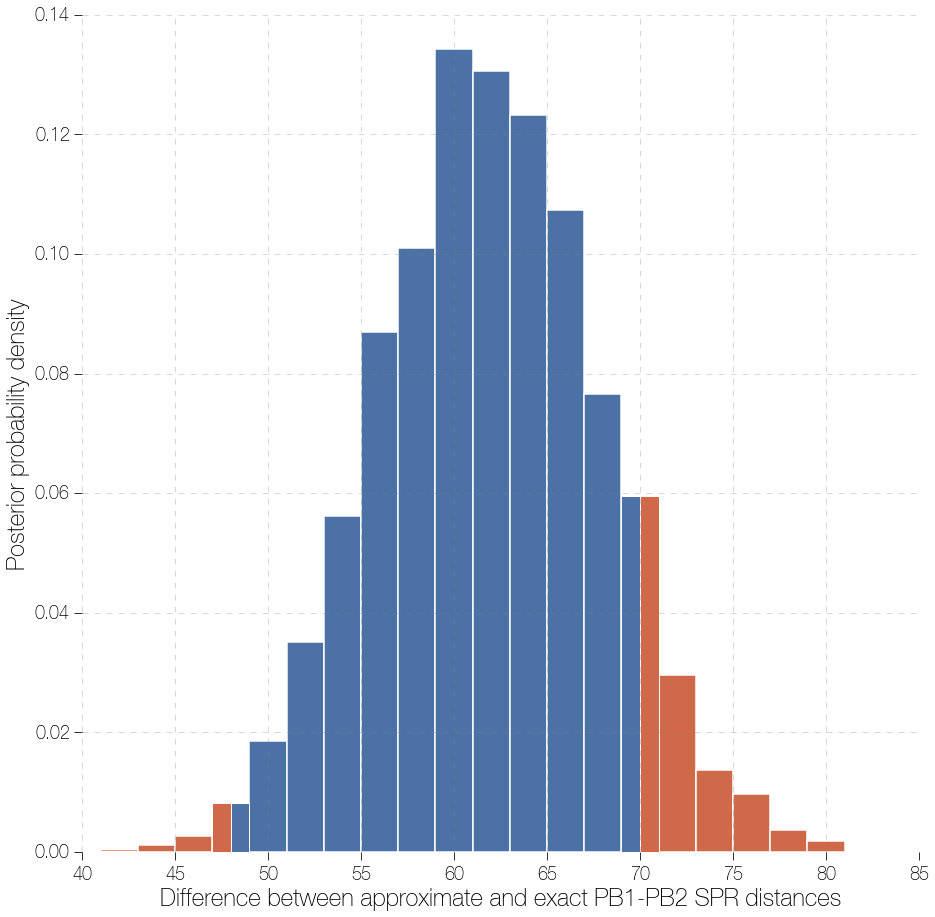
\includegraphics[width=0.65\textwidth]  {supp_figures/InfB_supp_PB1-PB2_hist.png}
%\caption{\textbf{Distribution of differences between exact and approximate PB1-PB2 SPR distances.}}
%\label{SPR_PB1-PB2_difference}
%\end{figure}

%\begin{figure}
%\centering  
%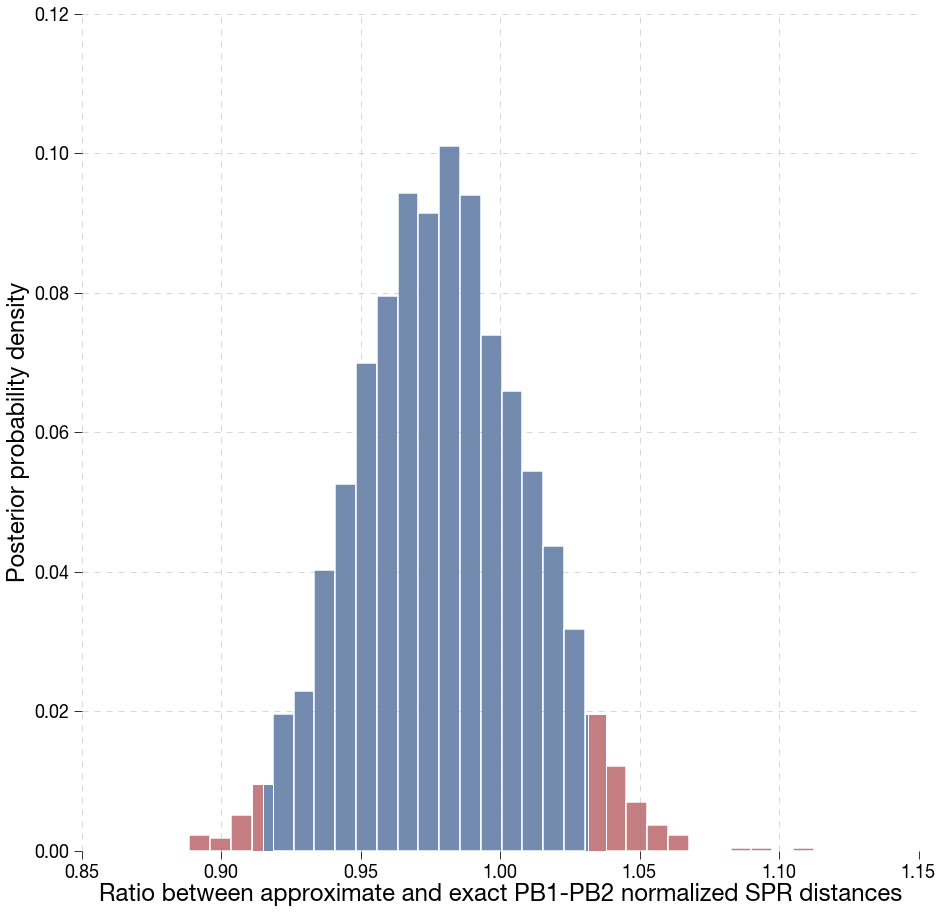
\includegraphics[width=0.65\textwidth]  {supp_figures/InfB_supp_PB1-PB2_hist2.png}
%\caption{\textbf{Distribution of ratios between exact and approximate PB1-PB2 SPR distances.}}
%\label{SPR_PB1-PB2_ratio}
%\end{figure}

%\begin{figure}
%\centering  
%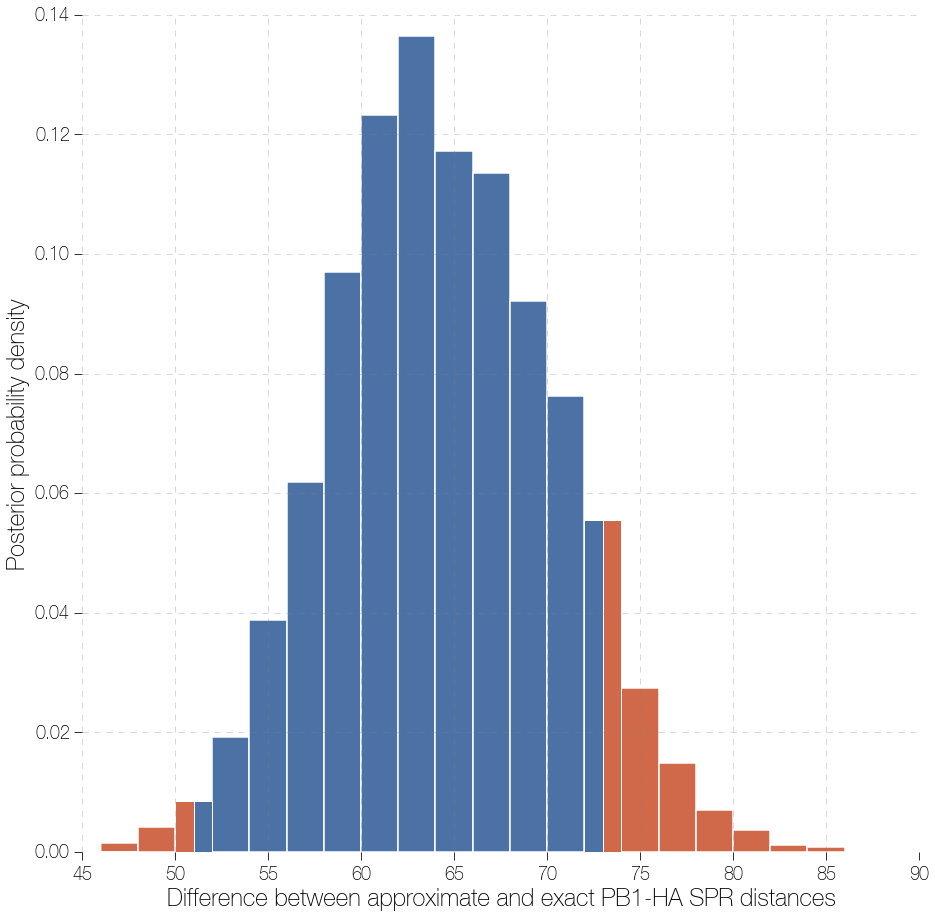
\includegraphics[width=0.65\textwidth]  {supp_figures/InfB_supp_PB1-HA_hist.png}
%\caption{\textbf{Distribution of differences between exact and approximate PB1-HA SPR distances.}}
%\label{SPR_PB1-HA_difference}
%\end{figure}

%\begin{figure}
%\centering  
%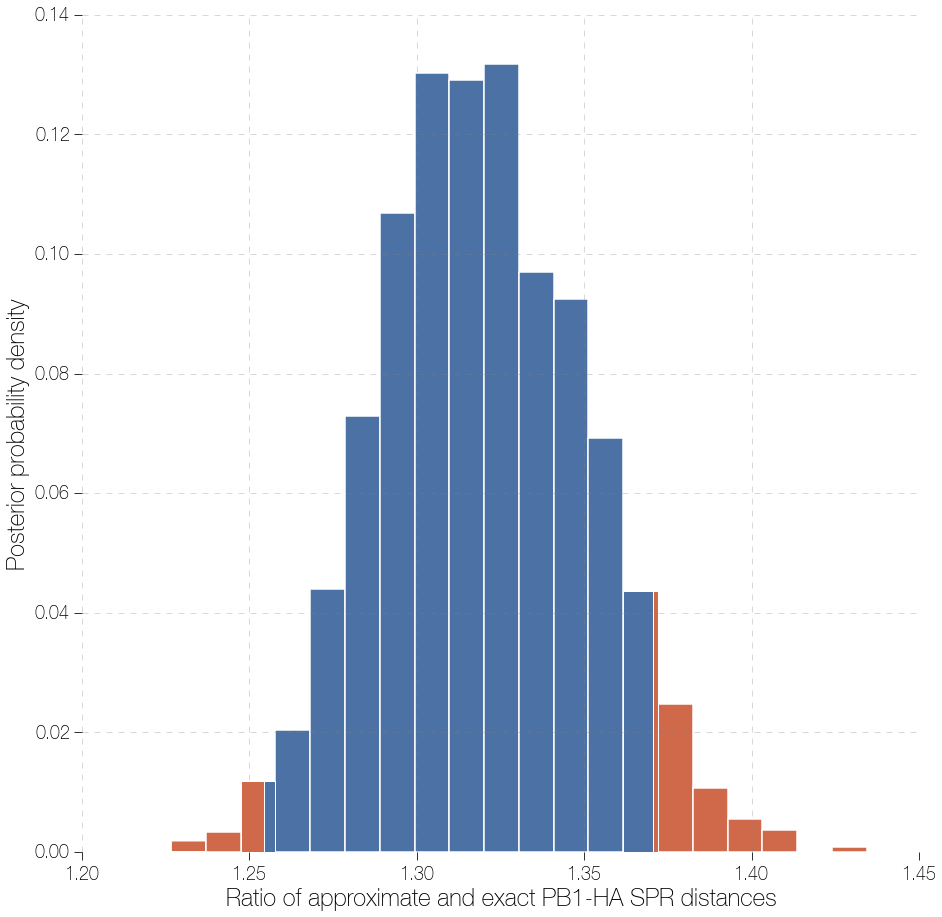
\includegraphics[width=0.65\textwidth]  {supp_figures/InfB_supp_PB1-HA_hist2.png}
%\caption{\textbf{Distribution of ratios between exact and approximate PB1-HA SPR distances.}}
%\label{SPR_PB1-HA_ratio}
%\end{figure}

%\begin{figure}
%\centering  
%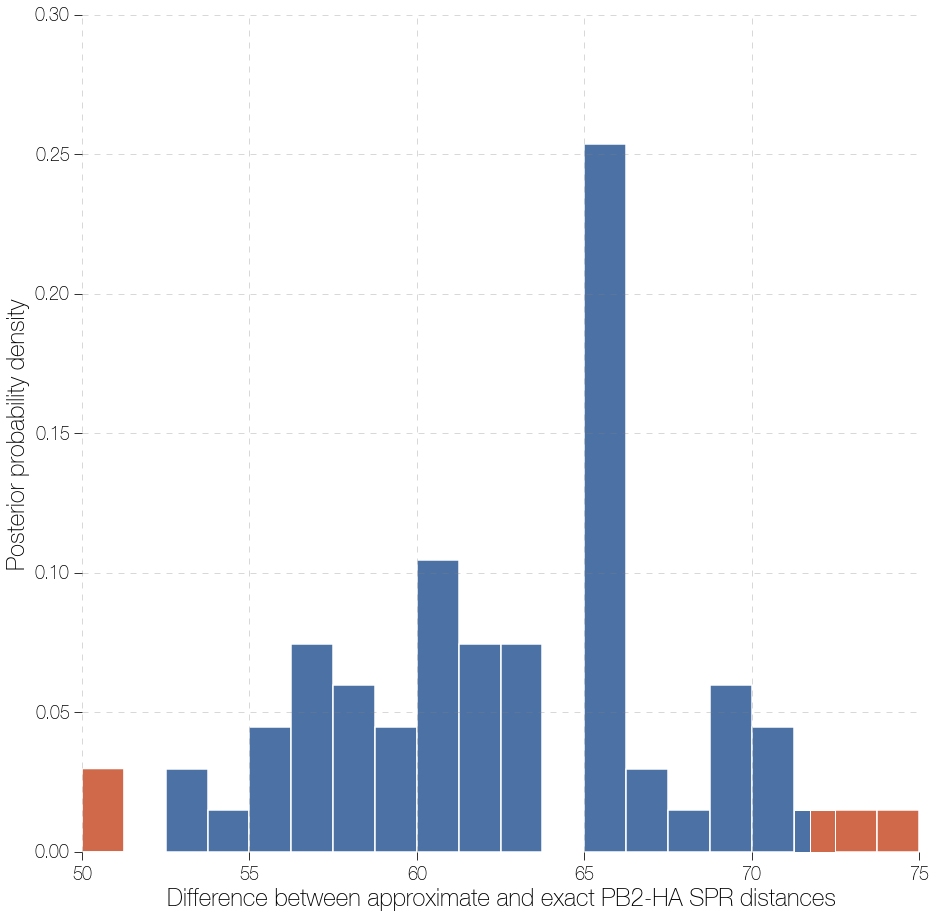
\includegraphics[width=0.65\textwidth]  {supp_figures/InfB_supp_PB2-HA_hist.png}
%\caption{\textbf{Distribution of differences between exact and approximate PB2-HA SPR distances.}}
%\label{SPR_PB2-HA_difference}
%\end{figure}

%\begin{figure}
%\centering  
%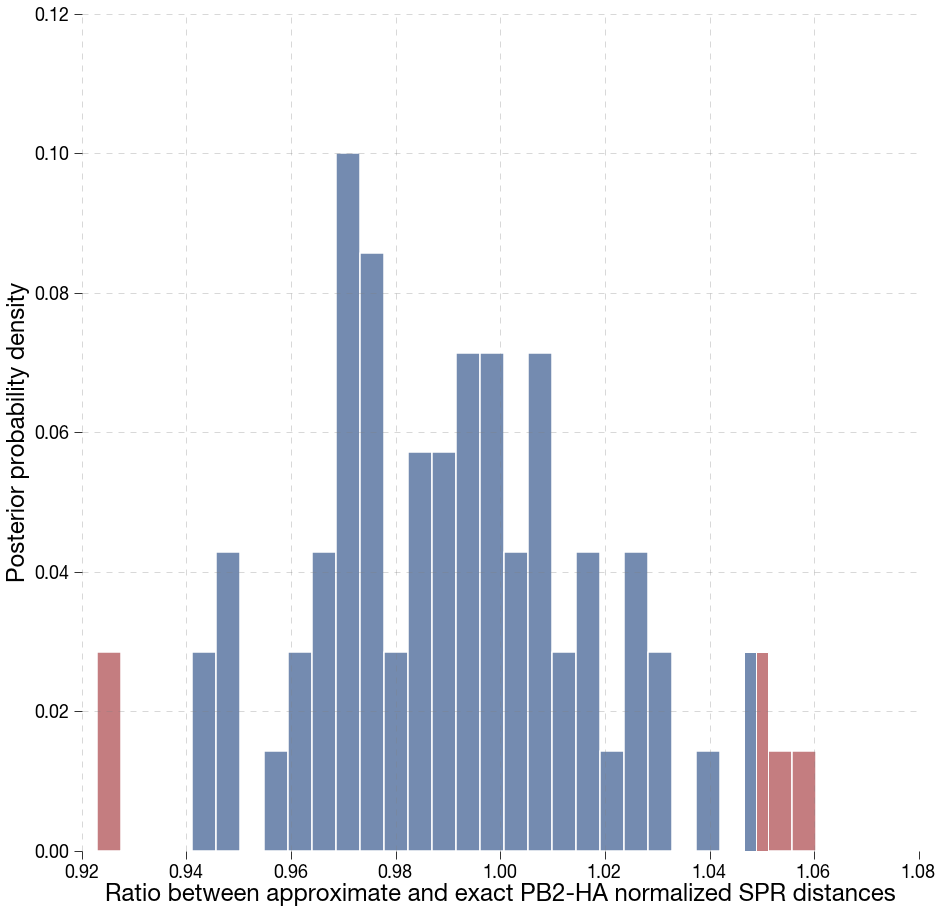
\includegraphics[width=0.65\textwidth]  {supp_figures/InfB_supp_PB2-HA_hist2.png}
%\caption{\textbf{Distribution of ratios between exact and approximate PB2-HA SPR distances.}}
%\label{SPR_PB2-HA_ratio}
%\end{figure}

%\begin{figure}
%\centering  
%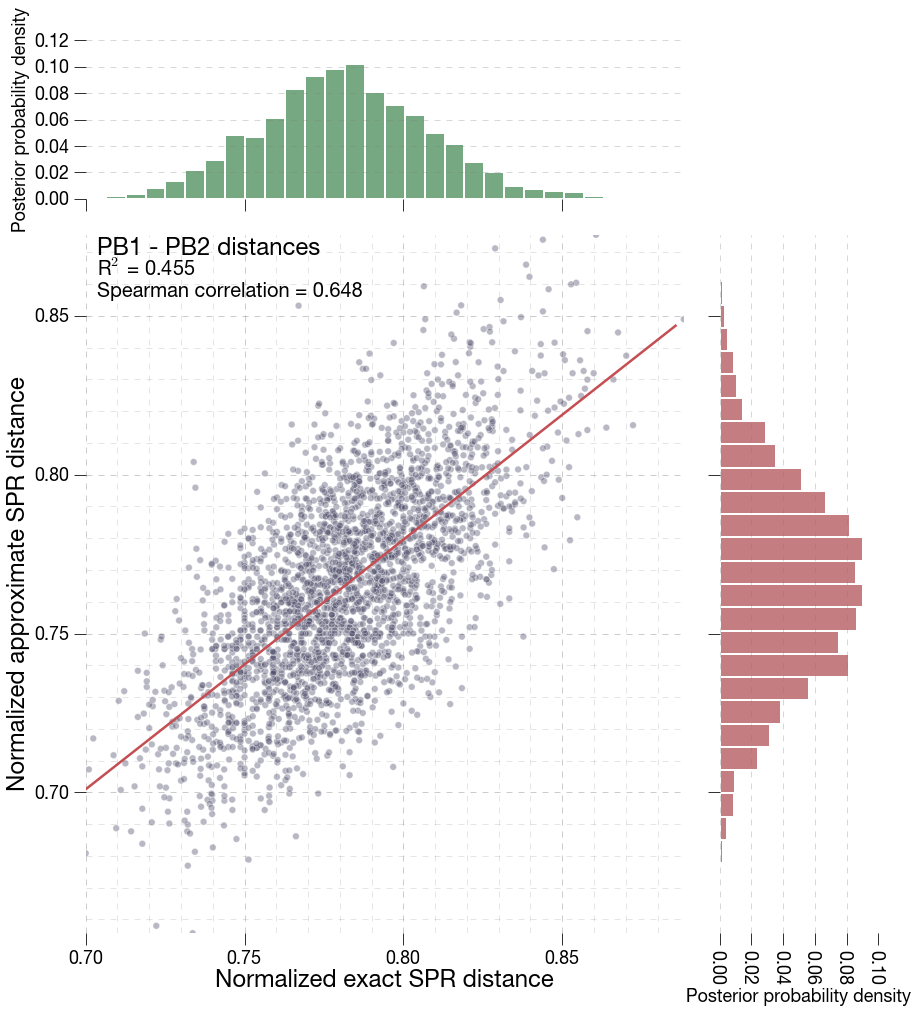
\includegraphics[width=0.4\textwidth]  {supp_figures/InfB_supp_PB1-PB2_corr.png}
%\caption{\textbf{Correlation between exact and approximate PB1-PB2 SPR distances.}}
%\label{SPR_PB1-PB2_correlation}
%\end{figure}

%\begin{figure}
%\centering  
%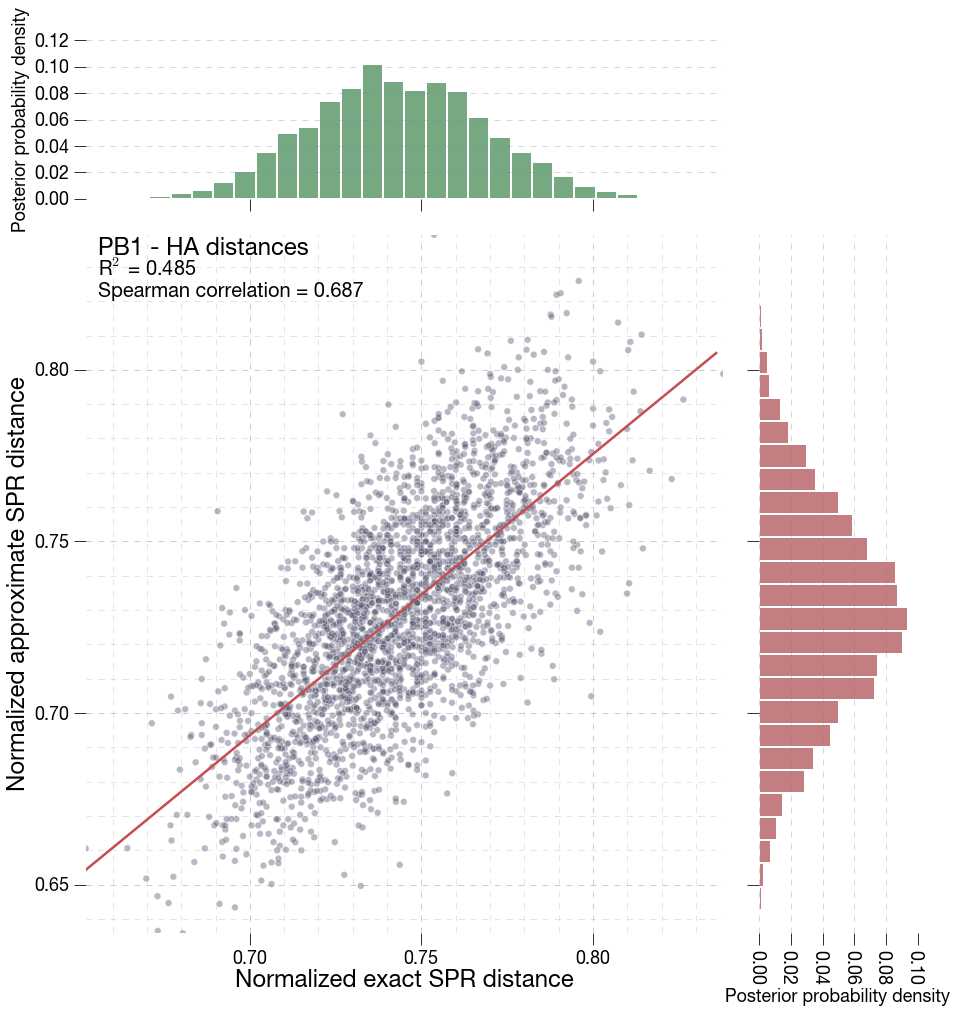
\includegraphics[width=0.4\textwidth]  {supp_figures/InfB_supp_PB1-HA_corr.png}
%\caption{\textbf{Correlation between exact and approximate PB1-HA SPR distances.}}
%\label{SPR_PB1-HA_correlation}
%\end{figure}

%\begin{figure}
%\centering  
%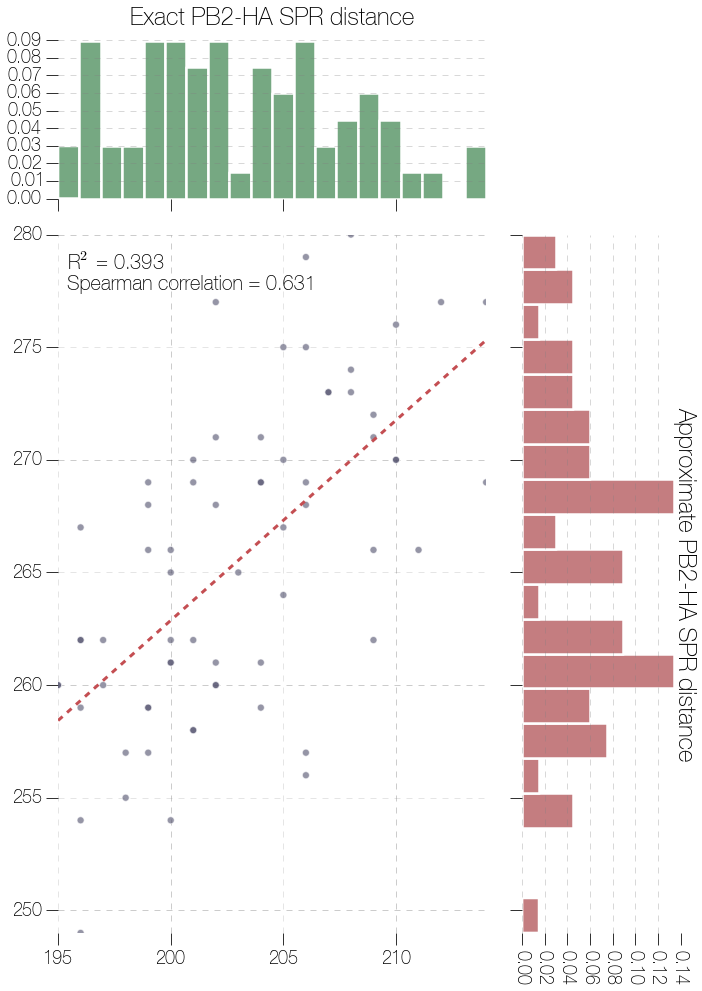
\includegraphics[width=0.4\textwidth]  {supp_figures/InfB_supp_PB2-HA_corr.png}
%\caption{\textbf{Correlation between exact and approximate PB2-HA SPR distances.}}
%\label{SPR_PB2-HA_correlation}
%\end{figure}

%\clearpage
%\section*{Multidimensional scaling}
%Figures \ref{MDSaaLD} and \ref{MDSntLD} visualize the relationships between segments based on mean amino acid and nucleotide site linkage disequilibrium estimates, respectively.
%PB1, PB2 and HA segments appear to be by far the most similar segments, as indicated by their proximity in the MDS embedding.
%Figures \ref{MDSaaCorr} and \ref{MDSntCorr} compare the observed mean LD values between segments. 
%Based on mean amino acid site LD (Figure \ref{MDSaaCorr}) only PB1, PB2 and HA segments show considerable clustering, all other segments being equidistant from each other in the MDS embedding.
%MDS distance versus mean nucleotide site LD scatter plot, on the other hand, shows a continuum of relationships between segments, which is probably caused by more variability at the nucleotide level than the amino acid level.
%This difference in variability would build up linkage disequilibrium between nucleotide sites and would reduce it via convergent substitutions over relatively short periods of time.

%\begin{figure}
%\centering  
%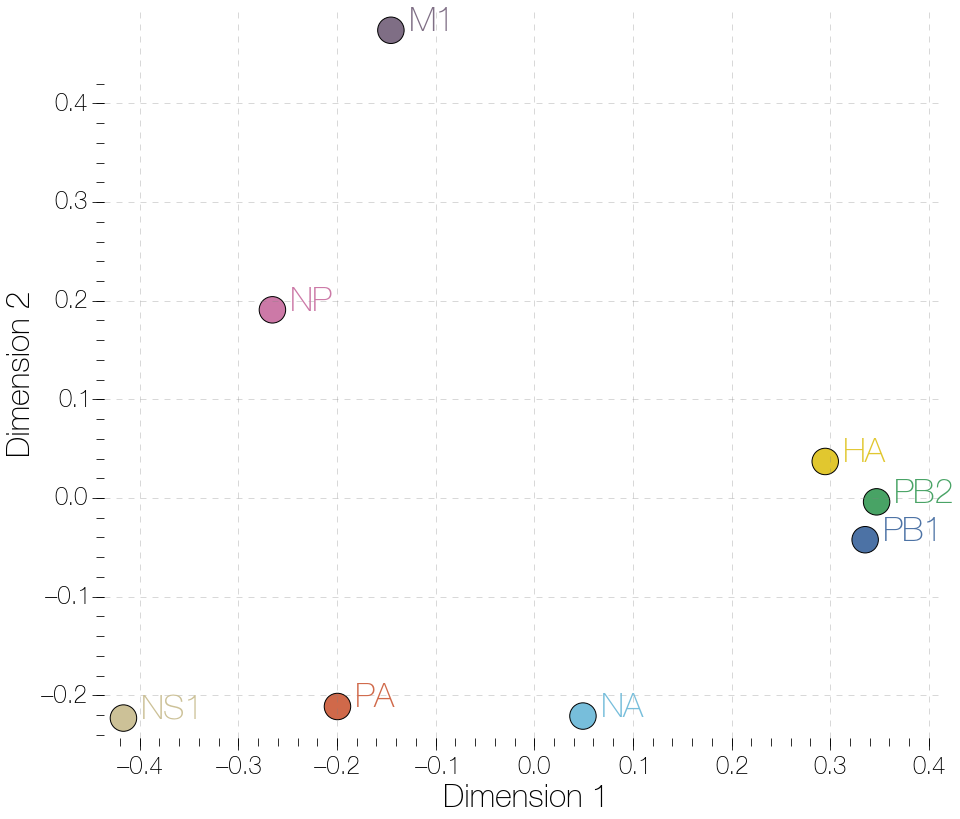
\includegraphics[width=0.65\textwidth]  {supp_figures/InfB_8x8_aaLD_MDS.png}
%\caption{\textbf{2-dimensional MDS embedding of influenza B virus segments based on mean amino acid linkage disequilibrium ($\chiSq$).}}
%\label{MDSaaLD}
%\end{figure}

%\begin{figure}
%\centering  
%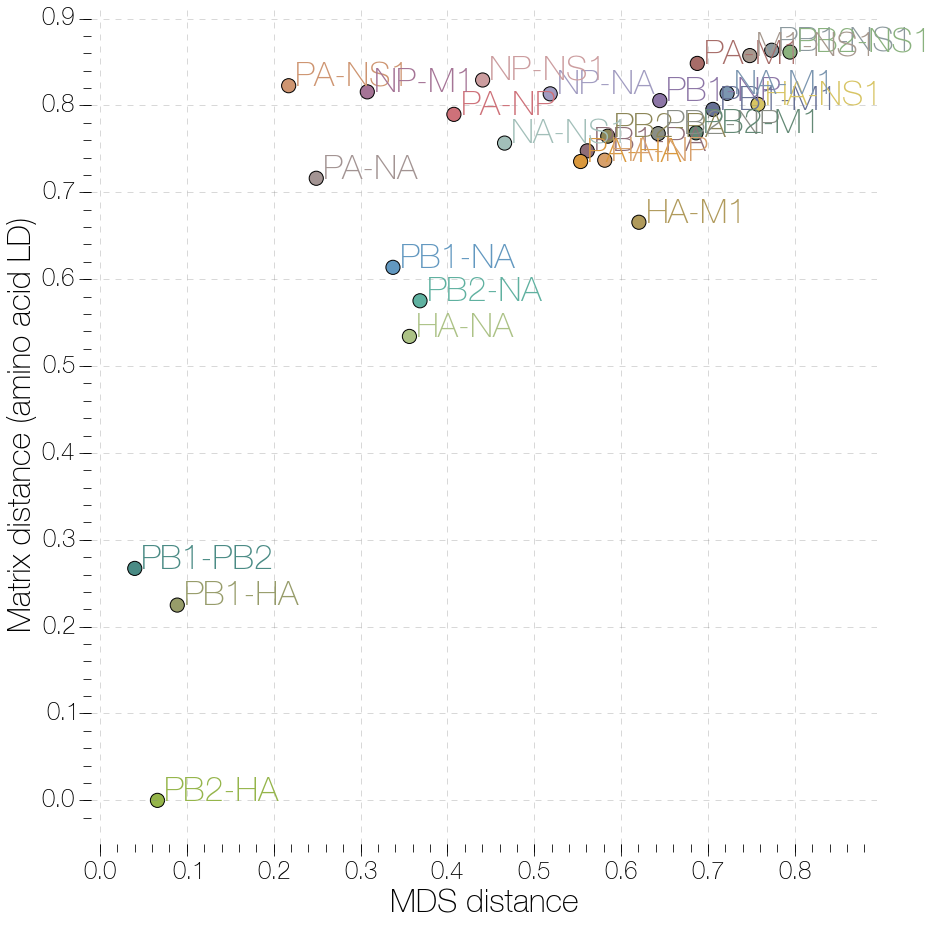
\includegraphics[width=0.65\textwidth]  {supp_figures/InfB_aaLD_MatrixMDScorr.png}
%\caption{\textbf{Correlation between mean amino acid site linkage disequilibrium and MDS embedding distance for all pairs of segments.}}
%\label{MDSaaCorr}
%\end{figure}

%\begin{figure}
%\centering  
%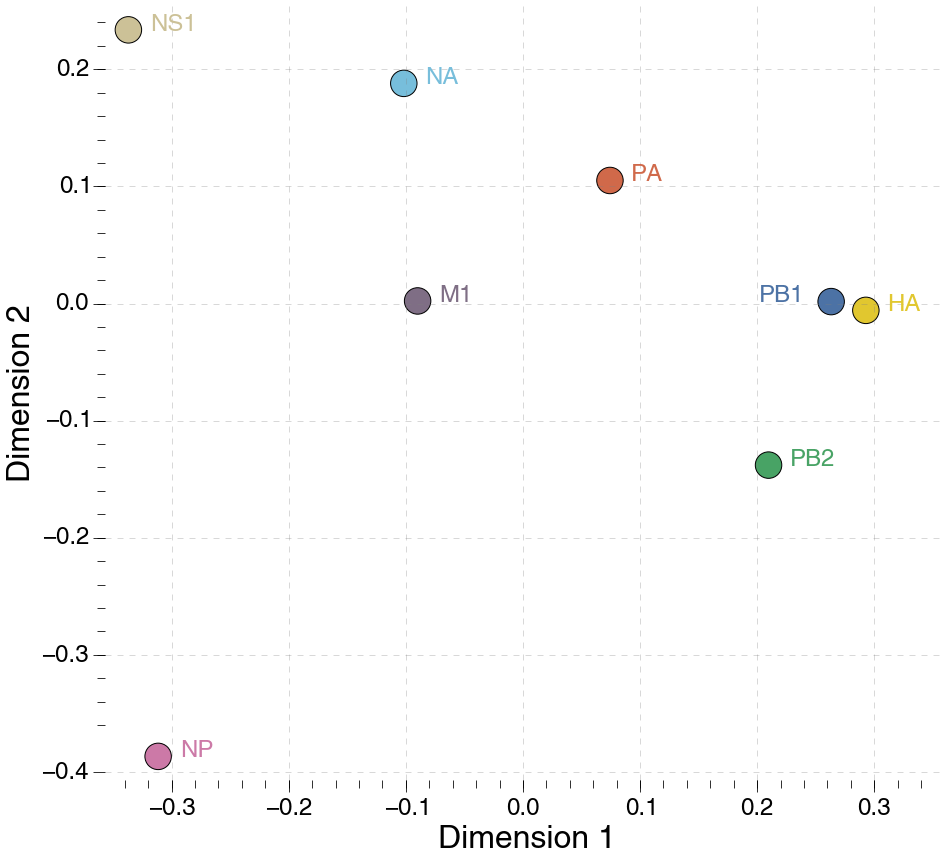
\includegraphics[width=0.65\textwidth]  {supp_figures/InfB_8x8_ntLD_MDS.png}
%\caption{\textbf{2-dimensional MDS embedding of influenza B virus segments based on mean nucleotide linkage disequilibrium ($\chiSq$).}}
%\label{MDSntLD}
%\end{figure}

%\begin{figure}
%\centering  
%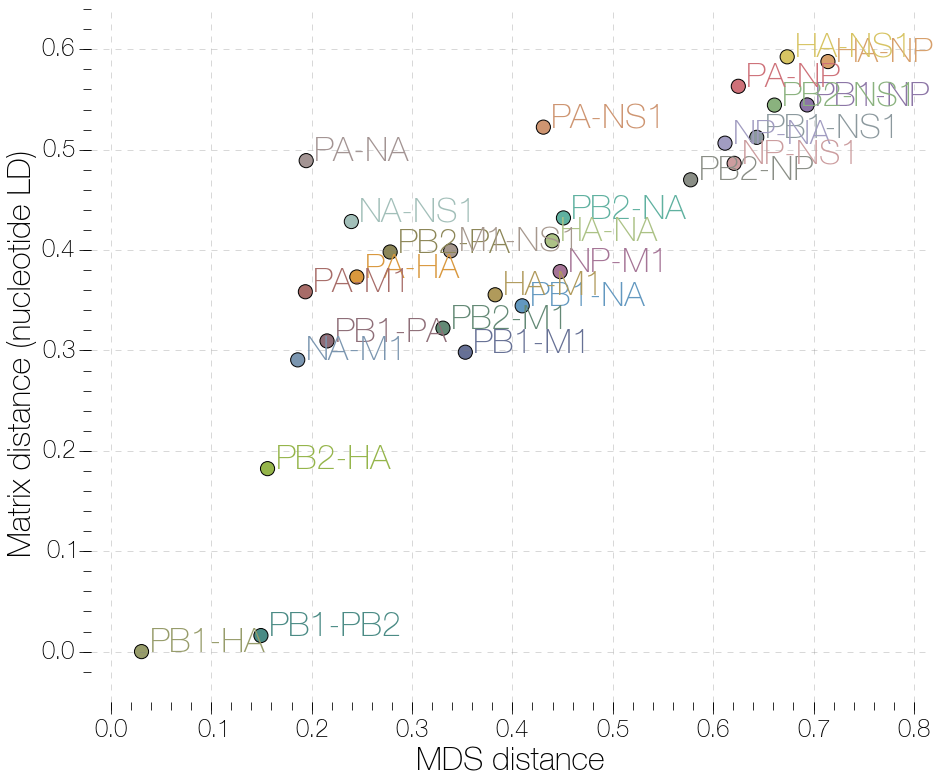
\includegraphics[width=0.65\textwidth]  {supp_figures/InfB_ntLD_MatrixMDScorr.png}
%\caption{\textbf{Correlation between mean nucleotide site linkage disequilibrium and MDS embedding distance for all pairs of segments.}}
%\label{MDSntCorr}
%\end{figure}

%\section*{Differences between Vic and Yam PB1-PB2-HA}
%Through the combination of inferred PB1-PB2-HA background and realized synonymous and non-synonymous substitution counts on branches \citep{obrien2009} it was possible to investigate whether Victoria and Yamagata lineage backgrounds differ in substitution rates.
%Figure \ref{robustCounting} shows the inferred synonymous, non-synonymous (both as substitutions per year) and overall nucleotide substitution rate (as substitutions per site per year) under different lineages of PB1-PB2-HA.

%\begin{figure}
%\centering  
%\includegraphics[width=0.65\textwidth]  {supp_figures/InfB_lineageRatios.png}
%\caption{\textbf{Total counts and ratios of Victoria and Yamagata lineage sequences in each segment.}}
%\label{lineageRatios}
%\end{figure}

\clearpage

\bibliographystyle{mbe}
\bibliography{fluB}

\end{document}